\documentclass[a4paper, 11pt, oneside]{book} % Setting the type of document.

\usepackage{amssymb,amsmath,amsthm} % Enhancing maths environments. 

\usepackage{indentfirst} % Indent the first paragraph of each section.

\usepackage[no-math]{fontspec} % Load the OpenFont to the LaTeX, without modifying maths environments.

\defaultfontfeatures{Mapping=tex-text}
% In LaTeX, we use `` and '' as quotation mark, use -, --, --- as different lines. The compiler will automatically process that. These marks are called 'tex-text.'

\usepackage{xltxtra} 
% xltxtra: Provide a number of small features that are useful for XeLaTeX.
% polyglossia: Modern multilingual typesetting with XeLaTeX.

% \usepackage{titlesec} % Select alternative section titles format. 
% \titleformat{\chapter}{\LARGE\bf}{\thechapter}{1em}{}
% \titlespacing*{\chapter}{0pt}{3.5ex plus 1ex minus .2ex}{2.3ex plus .2ex}

\parskip=0pt plus 1pt % Setting paragraph skip distance.

% Setting "no separation" between items in itemize/enumerate.
\usepackage{enumitem}
\setlist{nosep}

% Import footnote package.
\usepackage[stable]{footmisc}

% Set the distance between text and math environments.
\makeatletter
\g@addto@macro\normalsize{%
  \setlength\abovedisplayskip{10pt}
  \setlength\belowdisplayskip{10pt}
  \setlength\abovedisplayshortskip{10pt}
  \setlength\belowdisplayshortskip{10pt}
}
\makeatother

% --------------- LANGUAGE SETTING --------------- 
\XeTeXlinebreaklocale "th_TH" 
\XeTeXlinebreakpenalty = 100
\XeTeXlinebreakskip = 0pt plus 1pt
\linespread{1.5}
% For Thai, I recommend to scale the size to the uppercase size of latin alphabet
\setmainfont[Scale=MatchUppercase,Mapping=tex-text]{TH Sarabun New}
% Because latin font in Sarabun is Sans Serif, we prefer to use Serif font
\newfontfamily{\thaifont}[Scale=MatchUppercase,Mapping=tex-text]{TH Sarabun New}
% --------------- LANGUAGE SETTING --------------- 

\usepackage[top=2.54cm, bottom=2.54cm, left=2.38cm, right=1.9cm]{geometry} % Set the margins of all pages.

%--------Start of Code Snipplet Setting------------%
\usepackage{listings}
\usepackage{xcolor}

\definecolor{codegreen}{rgb}{0,0.6,0}
\definecolor{codegray}{rgb}{0.5,0.5,0.5}
\definecolor{codepurple}{rgb}{0.58,0,0.82}
\definecolor{backcolour}{rgb}{0.95,0.95,0.92}

\lstdefinestyle{mystyle}{
    backgroundcolor=\color{backcolour},   
    commentstyle=\color{codegreen},
    keywordstyle=\color{magenta},
    numberstyle=\tiny\color{codegray},
    stringstyle=\color{codepurple},
    basicstyle=\ttfamily\footnotesize,
    breakatwhitespace=false,         
    breaklines=true,                 
    captionpos=b,                    
    keepspaces=true,                 
    numbers=left,                    
    numbersep=5pt,                  
    showspaces=false,                
    showstringspaces=false,
    showtabs=false,                  
    tabsize=1,
    numberstyle=\ttfamily\tiny,
    breakindent = 0pt
}

\lstset{style=mystyle}
%--------End of Code Snipplet Setting------------%

\usepackage{textgreek} % Greek letters in text environment.

\usepackage{gensymb} % Generic symbols for both text and math environments.

\usepackage{hyperref} % Hyperreference in LaTeX.

\usepackage{siunitx} % SI units in LaTeX.
\sisetup{detect-all} 

\usepackage{cite} % Using BibTeX file for declaring references.

\usepackage{setspace} % set singlespace around code listings.

% Change chapter, figure and contents headers to Thai.
\renewcommand{\chaptername}{บทที่}
\renewcommand{\figurename}{รูปที่}
\renewcommand{\contentsname}{สารบัญ}
\renewcommand\bibname{เอกสารอ้างอิง}

% Path to graphics.
\graphicspath{ {./images/} }

\begin{document}

\title{รายงานการฝึกงาน}
\author{นาย ณัฐชนน จริยานุรัตน์}

\frontmatter % No page number here.

%----------------------------------------------------------------
\chapter*{คำนำ}

รายงานนี้นำเสนอการออกแบบวงจร Op Amp แบบ Two-Stage Amplifier โดยให้ใช้โปรแกรม LTSpice ในการจำลองและทดสอบวงจรไฟฟ้า และใช้โมเดล CMOS แบบ BSIM3 เทคโนโลยี 0.18 nm ในการออกแบบวงจรดังกล่าว

\begin{flushright} 
    ณัฐชนน จริยานุรัตน์
\end{flushright}

\tableofcontents

\mainmatter % Page number come back here.

%----------------------------------------------------------------
\chapter{รายละเอียดงาน}

\section{การออกแบบวงจร Op Amp แบบ Two-Stage Amplifier}

Op Amp เป็นส่วนประกอบที่ใช้บ่อยในวงจรอิเล็กทรอนิกส์ต่าง ๆ สำหรับ Op Amp ที่สามารถออกแบบได้ง่ายและเป็นพื้นฐานมากที่สุด คือวงจรแบบ Two-Stage Amplifier

\subsection{ทฤษฎีที่เกี่ยวข้อง}

\subsubsection{โครงสร้างทั่วไปของวงจร Two-Stage Amplifier}

\begin{figure}[h]
    \centering
    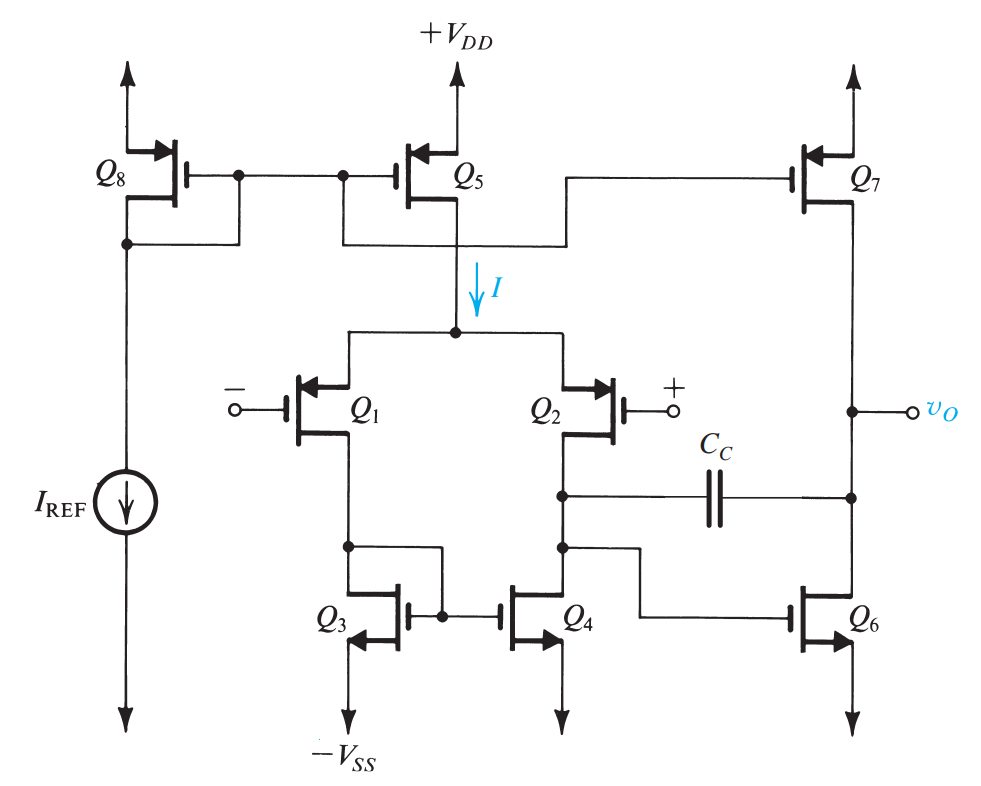
\includegraphics[width=10cm]{opamp-twostage}
    \caption{โครงสร้างทั่วไปของวงจร two-stage CMOS op-amp (จาก Sedra and Smith, Microelectronic Circuits, 7E \cite{Sedra15})}
    \label{opamp-twostage}
\end{figure}

จากรูปที่~\ref{opamp-twostage} จะเห็นได้ว่า วงจร Two-Stage Amplifier จะประกอบไปด้วยสามส่วนหลัก ได้แก่ 

\begin{itemize}
    \item วงจร Differential Amplifier ซึ่งประกอบไปด้วยทรานซิสเตอร์คือ Q1, Q2, Q3 และ Q4 ซึ่งทำหน้าที่ขยายสัญญาณในส่วนแรก โดยสัญญาณขาเข้าจะเข้ามาทางสัญลักษณ์ + และ - ในรูป
    \item หลังจากนั้น สัญญาณขาออกจากวงจร Differential Amplifier จะไปเข้าสู่วงจร Common-Source Amplifier ซึ่งประกอบไปด้วยทรานซิสเตอร์ Q6 ซึ่งทำหน้าที่ขยายสัญญาณในขั้นสุดท้าย
    \item วงจร Current Mirror ประกอบไปด้วยทรานซิสเตอร์ Q5, Q7 และ Q8 ซึ่งสร้างกระแสอ้างอิงให้กับทั้งวงจร Differential Amplifier และวงจร Common-Source Amplifier 
\end{itemize}

\subsubsection{เงื่อนไขของการไบแอสวงจร}

เนื่องจาก drain-source voltage ของทรานซิสเตอร์ Q3, Q4 และ Q6 จะต้องเท่ากัน ดังนั้นกระแสที่ผ่านทานซิสเตอร์ทั้งสามตัวจะต้องเท่ากันด้วย เนื่องจากกระแสที่ผ่านทรานซิสเตอร์ Q3, Q4 จะเป็นครึ่งหนึ่งของกระแสที่ผ่านทรานซิสเตอร์ Q5 ดังนั้น อัตราส่วน W/L ของทรานซิสเตอร์ในรูปที่~\ref{opamp-twostage} จึงต้องมีค่าเป็น
\begin{equation}
    \frac{(W/L)_6}{(W/L)_4} = 2\frac{(W/L)_7}{(W/L)_5}
    \label{offset-eq}
\end{equation}

\subsubsection{ช่วงของสัญญาณขาเข้า (Input Common-Mode Range) และสัญญาณขาออก  (Output Swing)}

สำหรับช่วงของสัญญาณขาเข้า (Input Common-Mode Range) และสัญญาณขาออก  (Output Swing) ของวงจร two-stage CMOS op-amp เป็นดังนี้

ช่วงของสัญญาณขาเข้า (Input Common-Mode Range):
\begin{subequations}
    \label{input-range}
    \begin{align}
        \textrm{lower limit} &= -V_{SS} + V_{OV3} + V_{tn} - |V_{tp}| \\
        \textrm{upper limit} &= +V_{DD} - |V_{tp}| - |V_{OV1}| - |V_{OV5}|
    \end{align}
\end{subequations}

ช่วงของสัญญาณขาออก (Output Swing):
\begin{subequations}
    \label{output-swing}
    \begin{align}
        \textrm{lower limit} &= -V_{SS} + V_{OV6} \\
        \textrm{upper limit} &= +V_{DD} - |V_{OV7}|
    \end{align}
\end{subequations}

เพื่อทำให้ช่วงของสัญญาณขาเข้าและสัญญาณขาออกกว้างขึ้น การออกแบบวงจรควรพยายามที่จะทำให้กระแสไบแอสมีค่าต่ำ เพื่อทำให้ overdrive voltage ของทรานซิสเตอร์มีค่าต่ำลง

จากสมการ สังเกตว่าขอบบนของ Input Common-Mode Range นั้นถูกทำให้ลดลงอย่างมากจากขนาดของ $|V_{tp}|$ ที่คงที่

\subsubsection{โมเดลสัญญาณขนาดเล็ก (Small-Signal Model) ของวงจร}

\begin{figure}[h]
    \centering
    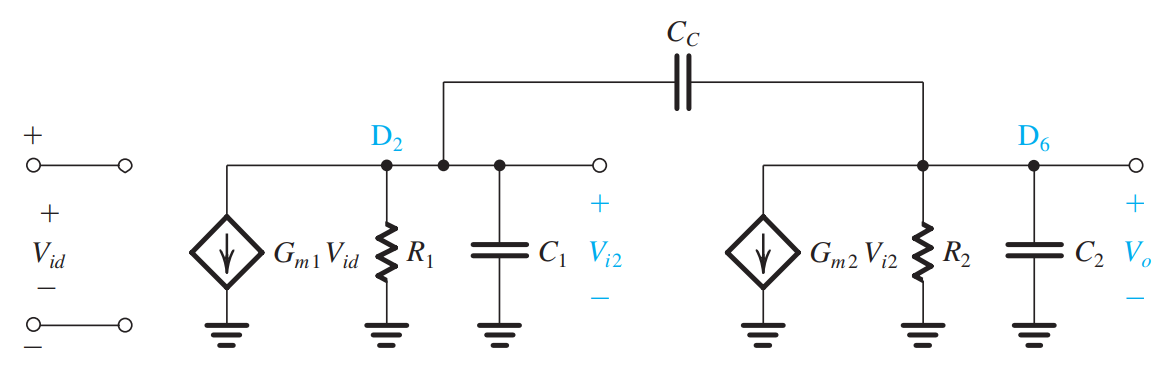
\includegraphics[width=\linewidth]{opamp-twostage-smallsignal}
    \caption{โมเดลสัญญาณขนาดเล็ก (Small-Signal Model) ของวงจรในรูปที่~\ref{opamp-twostage} (จาก Sedra and Smith, Microelectronic Circuits, 7E \cite{Sedra15})}
    \label{opamp-twostage-smallsignal}
\end{figure}

จากการคำนวณต่อจากรูปที่~\ref{opamp-twostage} จะได้ว่าโมเดลสัญญาณขนาดเล็กในรูปที่~\ref{opamp-twostage-smallsignal} จะมีค่าของตัวแปรขององค์ประกอบต่าง ๆ ดังนี้ คือ 
\begin{subequations}
    \begin{align}
        G_{m1} &= g_{m1} \\
        G_{m2} &= g_{m6} \\
        R_1 &= (r_{o2}||r_{o4}) \\
        R_2 &= (r_{o6}||r_{o7})
    \end{align}
\end{subequations}

\subsubsection{อัตราขยายของวงจร}

จากโมเดลสัญญาณขนาดเล็กในรูปที่~\ref{opamp-twostage-smallsignal} สามารถคำนวณหาอัตราขยายของ stage แรก คือ Differential Amplifier และ stage ที่สอง คือ Common-Source Amplifier ได้ดังนี้

อัตราขยายของ stage แรก: 
\begin{equation}
    A_1 = -g_{m1}(r_{o2}||r_{o4}) = -\frac{2}{|V_{OV1}|}/( \frac{1}{|V_{A2}|} + \frac{1}{|V_{A4}|} )
    \label{gain-1}
\end{equation}

อัตราขยายของ stage ที่สอง
\begin{equation}
    A_2 = -g_{m6}(r_{o6}||r_{o7}) = -\frac{2}{|V_{OV6}|}/( \frac{1}{|V_{A6}|} + \frac{1}{|V_{A7}|} )
    \label{gain-2}
\end{equation}

หากต้องการอัตราขยายของวงจรให้มากขึ้น สามารถทำได้โดยการลดกระแสไบแอสของทรานซิสเตอร์ลง จะทำให้ overdrive voltage ของทรานซิสเตอร์มีค่าลดลงตาม และทำให้อัตราขยายมากขึ้น (แต่จะแลกมาด้วยความต้านทานของสัญญาณรบกวนที่แย่ลง) ในขณะเดียวกัน การเพิ่ม Early voltage ของทรานซิสเตอร์โดยการเพิ่มความยาว (L) ของทรานซิสเตอร์ก็สามารถทำให้อัตราขยายของวงจรเพิ่มขึ้นเช่นกัน (แต่จะแลกมาด้วยขนาดวงจรที่เพิ่มขึ้น และวงจรจะใช้กระแสมากขึ้น ทำให้พลังงานที่ต้องใช้ในวงจรมากขึ้น)

\subsubsection{การตอบสนองเชิงความถี่ของวงจร}

จากรูปที่~\ref{opamp-twostage-smallsignal} จะได้ว่า $C_1$ คือความจุไฟฟ้าทั้งหมดตั้งแต่ขาออกของวงจรขยาย stage แรก จนถึง ground ของวงจร ดังนั้นจึงได้ว่า
\begin{equation}
    C_1 = C_{gd2} + C_{db2} + C_{gd4} + C_{db4} + C_{gs6}
    \label{C-1}
\end{equation}

เช่นเดียวกัน จะได้ว่า $C_1$ คือความจุไฟฟ้าทั้งหมดตั้งแต่ขาออกของวงจรขยาย stage ที่สอง จนถึง ground ของวงจร ดังนั้นจึงได้ว่า
\begin{equation}
    C_2 = C_{db6} + C_{db7} + C_{gd7} + C_{L}
    \label{C-2}
\end{equation}

โดยตัวแปรของความจุไฟฟ้าต่าง ๆ ในสมการ~\ref{C-1} และ~\ref{C-2} มีความหมายดังนี้ คือ

$C_L$ คือความจุไฟฟ้าของโหลดที่ต่อกับวงจรขาออก

$C_{gd}$ คือความจุไฟฟ้าของทรานซิสเตอร์ระหว่างขา gate และขา drain

$C_{gs}$ คือความจุไฟฟ้าของทรานซิสเตอร์ระหว่างขา gate และขา source

$C_{sb}$ คือความจุไฟฟ้าของทรานซิสเตอร์ระหว่างขา source และขา body

$C_{db}$ คือความจุไฟฟ้าของทรานซิสเตอร์ระหว่างขา drain และขา body

เลขหลัง subscript คือค่าของทรานซิสเตอร์ตามหมายเลขที่ระบุไว้ในรูปที่~\ref{opamp-twostage}

ตัวแปรความจุไฟฟ้าต่าง ๆ มีค่าเป็นดังนี้
\begin{subequations}
    \begin{align}
        C_{gd} &= WL_{ov}C_{ox} \\
        C_{gs} &= \frac{2}{3}WLC_{ox} + WL_{ov}C_{ox} \\
        C_{sb} &= C_{sb0}/\sqrt{1+\frac{|V_{SB}|}{V_0}} \\
        C_{db} &= C_{db0}/\sqrt{1+\frac{|V_{DB}|}{V_0}}
    \end{align}
\end{subequations}

โดย $C_{ox}$ คือความจุไฟฟ้าที่เกิดจากชั้นออกไซต์, $W$ และ $L$ คือความกว้างและความยาวของทรานซิสเตอร์ ตามลำดับ, $V_0$ คือ junction built-in voltage ซึ่งปกติมีค่าอยู่ระหว่าง 0.6 - 0.8 V, $L_{ov} \approx 0.05L - 0.1L$ คือความยาวที่ซ้อนกันระหว่าง gate และ source/drain substrate, $C_{sb0}$ และ $C_{db0}$ คือค่าของ $C_{sb}$ และ $C_{db}$ เมื่อ body-source/drain bias มีค่าเป็น 0 V ตามลำดับ

อ้างอิงจาก Sedra and Smith \cite{Sedra15} การวิเคราะห์วงจรแบบ node analysis ในรูปที่~\ref{opamp-twostage-smallsignal} จะทำให้ได้ transfer function $V_{o}/V_{id}$ ที่มีขั้ว (pole) ทั้งหมด 2 ตำแหน่ง และมีศูนย์ (zero) ที่อยู่บน right complex plane ทั้งหมดหนึ่งตำแหน่ง ซึ่งมีค่าดังนี้
\begin{subequations}
    \begin{align}
        \omega_{Z} &= \frac{G_{m2}}{C_{C}} \\
        \omega_{P1} &= \frac{1}{R_1[C_1+C_C(1+G_{m2}R_2)] + R_2(C_2+C_C)} \\
        \omega_{P2} &= \frac{G_{m2}C_C}{C_1C_2 + C_C(C_1+C_2)}
    \end{align}
\end{subequations}

โดยที่ขั้ว $\omega_{P1}$ จะมีค่าต่ำลงเนื่องจาก $C_C$ ดังนั้น $C_C$ จะช่วยเพิ่ม phase margin ของผลตอบสนองเชิงความถี่โดยการเลื่อน crossover frequency ให้ต่ำลงมาอยู่ที่ช่วงที่มี phase response สูง 

การประมาณค่าต่าง ๆ ในสมการที่ผ่านมาจะทำให้ได้ค่าที่จัดการได้ง่ายขึ้น ดังนี้
\begin{subequations}
    \label{pole-zero-approx}
    \begin{align}
        \omega_{Z} &= \frac{G_{m2}}{C_{C}} \\
        \omega_{P1} &= \frac{1}{R_1C_CG_{m2}R_2} \\
        \omega_{P2} &= \frac{G_{m2}}{C_2}
    \end{align}
\end{subequations}

ปัญหาของการลดลงของ phase response เนื่องจากการมีอยู่ของ zero ซึ่งอยู่บน right complex plane สามารถแก้ไขได้โดยการต่อความต้านทาน $R$ แบบอนุกรมกับตัวเก็บประจุ $C_C$ ซึ่งจะทำให้ $\omega_{Z}$ มีค่าที่เปลี่ยนไปเป็น
\begin{equation}
    \omega_{Z} = \frac{1}{C_{C}(\frac{1}{G_{m2}} - R)}
    \label{new-zero}
\end{equation}

หากทำให้ค่า $R$ มีค่าสูงขึ้นมากพอ จะทำให้ $\omega_{Z}$ เปลี่ยนไปอยู่ในฝั่งของ left complex plane แทน และทำให้ผลตอบสนองของ phase response เปลี่ยนเป็นการมีค่ามากขึ้นที่ตำแหน่งศูนย์ดังกล่าว

ไม่ว่าอย่างไรก็ตาม การต่อ $R$ แบบอนุกรมกับตัวเก็บประจุ $C_C$ ทำให้เกิด pole ขึ้นมาใหม่หนึ่งตำแหน่งในช่วงความถี่สูง ซึ่ง pole ใหม่นี้จะมีค่าเป็น
\begin{equation}
    \omega_{P3} = \frac{1}{RC_{1}}
    \label{new-pole}
\end{equation}

\begin{figure}[h]
    \centering
    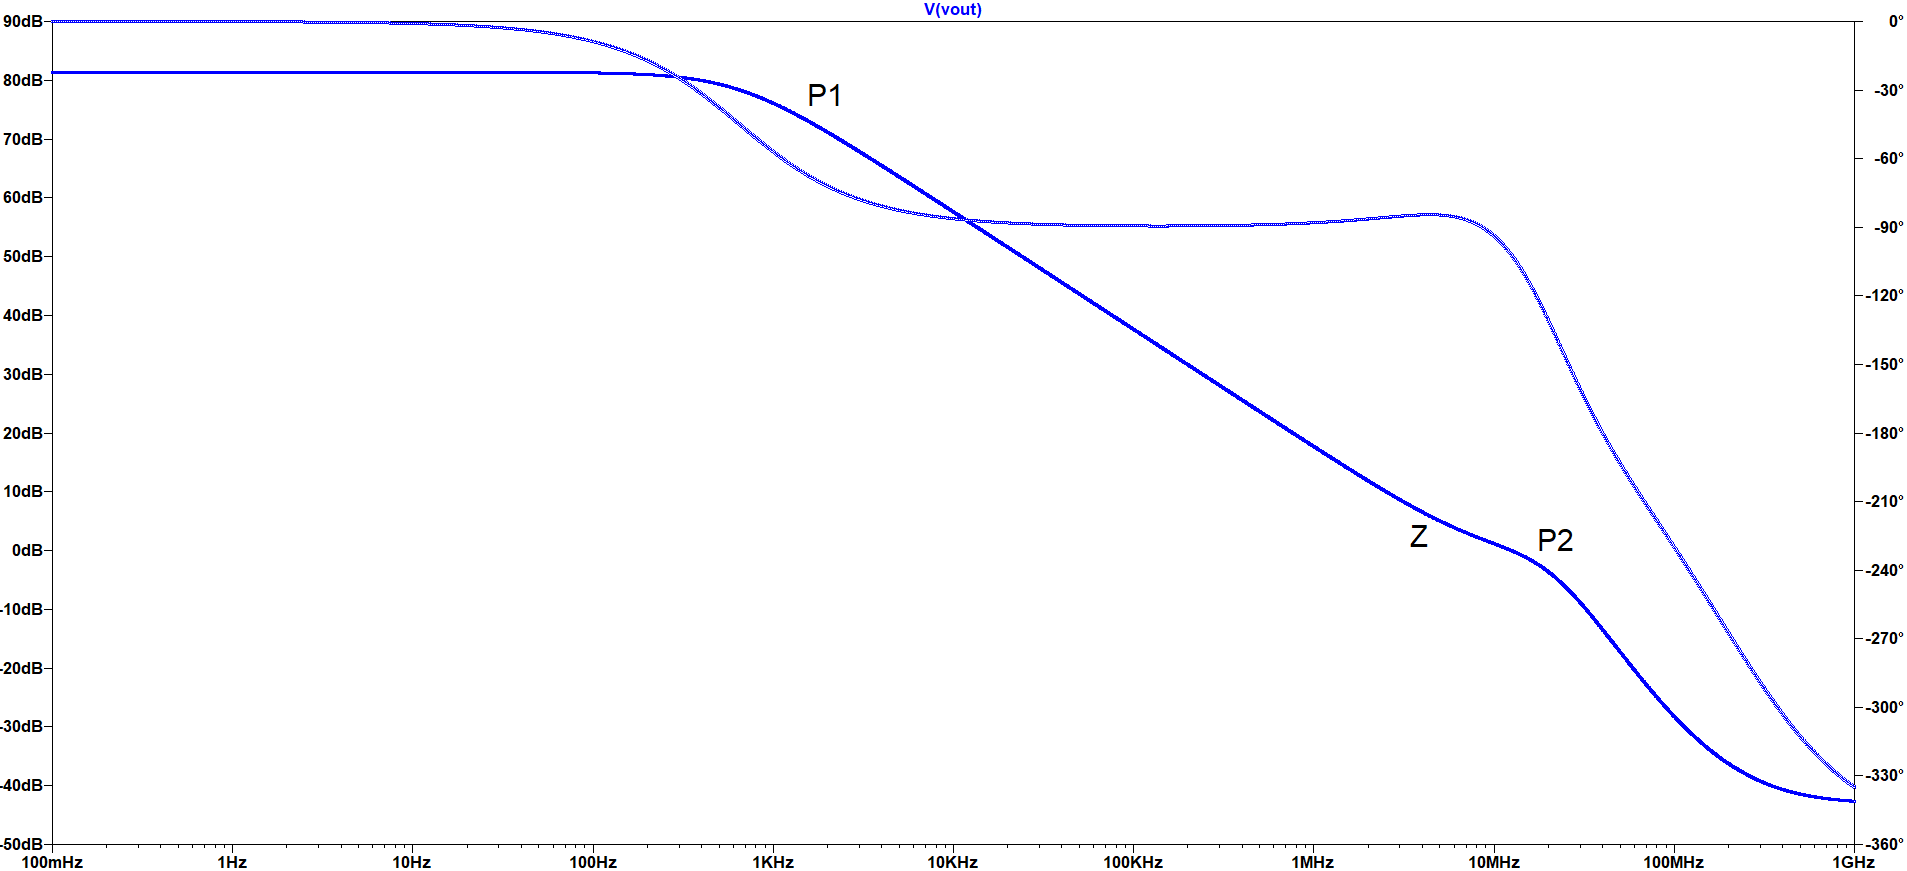
\includegraphics[width=\linewidth]{openloopgain_freqresponse}
    \caption{ผลตอบสนองเชิงความถี่ของ two-stage opamp ในกรณีที่ศูนย์ของผลตอบสนองเลื่อนมาอยู่ที่ left complex plane แล้ว โดยสังเกตเห็นว่าศูนย์ ($\omega_{Z}$) ดังกล่าวจะทำให้ phase response ของวงจรเพิ่มขึ้น ก่อนที่จะลดลงอย่างมากเมื่อผ่านความถี่ของขั้วตำแหน่งที่สอง ($\omega_{P2}$)}
    \label{openloopgain_freqresponse}
\end{figure}

\subsubsection{Slew Rate}

หากสัญญาณขาเข้าของวงจร op amp เปลี่ยนไปอย่างกะทันหัน สัญญาณขาออกของวงจร op amp จะไม่เปลี่ยนแปลงทันทีทันใด แต่จะค่อย ๆ เปลี่ยนจนกระทั่งถึงจุดคงตัว (steady-state) ความเร็วในช่วงระยะเวลาของการเปลี่ยนแปลงนั้นเรียกว่า Slew Rate

\begin{figure}[h]
    \centering
    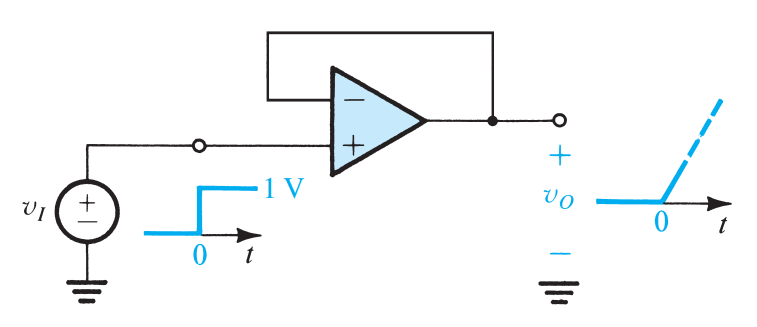
\includegraphics[width= 10cm]{slew_rate}
    \caption{แสดงนิยามโดยคร่าวของ Slew Rate (จาก Sedra and Smith, Microelectronic Circuits, 7E \cite{Sedra15})}
    \label{slew_rate}
\end{figure}

สำหรับการแปลงวงจร two-stage amplifier ให้อยู่ในรูปอย่างง่ายพอที่จะสามารถคำนวณ slew rate ได้โดยคร่าว ได้แสดงในรูปที่~\ref{opamp_as_integrator} ซึ่งเป็นการประมาณให้ stage ที่สองอยู่ในรูปของ integrator

\begin{figure}[h]
    \centering
    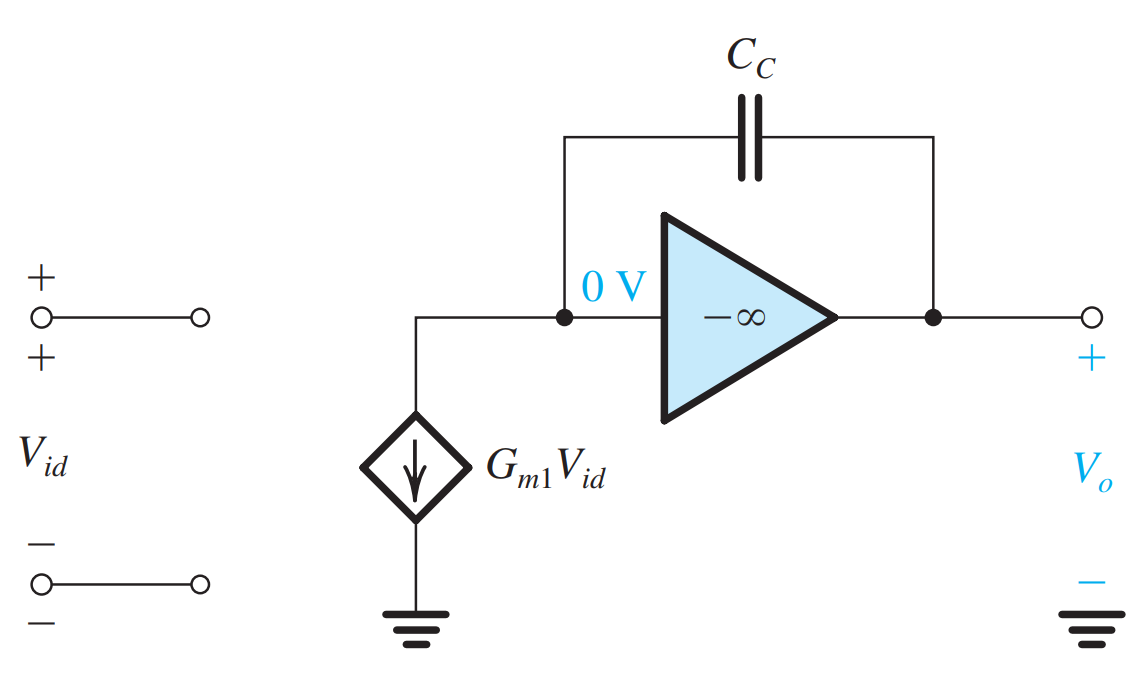
\includegraphics[width = 10cm]{opamp_as_integrator}
    \caption{2-stage op amp ที่ทำให้อยู่ในรูปอย่างง่าย}
    \label{opamp_as_integrator}
\end{figure}

เมื่อสัญญาณขาเข้าด้านหนึ่งของวงจรเปลี่ยนแปลงไป อีกด้านของ differential amplifier จะถูกปิดลง จึงไม่มีกระแสที่ไหลผ่านทรานซิสเตอร์ $Q_2$ หลังจากนั้น current mirror จะดึงกระแสจาก $C_C$ เข้ามาที่ทรานซิสเตอร์ $Q_2$ แทน จากวงจร integrator อย่างง่ายในรูปที่~\ref{opamp_as_integrator} จึงสามารถคำนวณได้ว่า 
\begin{equation}
    v_o(t) = (I/C_C)t
\end{equation}

โดยที่ $I$ คือกระแสจากทรานซิสเตอร์ $Q_4$ ดังนั้น slew rate หรือ SR จะมีค่าเป็น
\begin{equation}
    SR = I/C_C 
    \label{slew-eq}
\end{equation}

จากสมการดังกล่าวจึงได้ว่า ค่าของ $C_C$ ไม่ควรมีค่ามาก เนื่องจากจะทำให้ slew rate ลดลง

\subsubsection{สัญญาณรบกวนอ้างอิงขาเข้า (Input-Refer Noise) ของ MOSFET}

\begin{figure}[h]
    \centering
    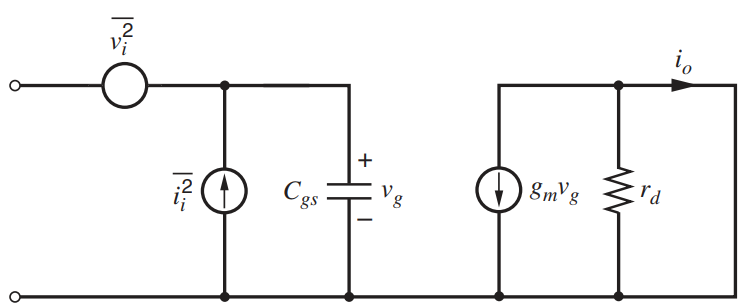
\includegraphics[width = 10cm]{MOS_noise_inputrefer}
    \caption{โมเดลสัญญาณขนาดเล็กของ MOSFET ที่พิจารณาถึงสัญญาณรบกวนอ้างอิงขาเข้าแบบแรงดัน (voltage) และกระแส (current) ร่วมด้วย (จาก Gray et. al., Analysis and Design of Analog Integrated Circuits, 5E \cite{Grey09})}
    \label{MOS_noise_inputrefer}
\end{figure}

จากรูปที่~\ref{MOS_noise_inputrefer}, Gray et. al. \cite{Grey09} ได้คำนวณแล้วว่าสัญญาณรบกวนอ้างอิงขาเข้าเชิงแรงดัน (voltage) จะมีค่าเป็นดังนี้
\begin{equation}
    \frac{\bar{v_i^2}}{\Delta f} = \frac{8kT}{3g_m} + \frac{K_f}{WLC_{ox}f} \label{Eq_MOS_noise}
\end{equation}

โดยที่ $k$ คือค่าคงที่โบลทซ์มานน์ (Boltzmann constant), และ $K_f$ ค่าคงที่ของ flicker noise ซึ่งโดยทั่วไปจะมีค่าประมาณ \num{3e-12} \si{V^2.\pico F}

ในสมการที่~\ref{Eq_MOS_noise} พจน์แรกคือ thermal noise และพจน์ที่สองคือ flicker noise (หรือ 1/f noise) โดยสัญญาณรบกวนในสมการดังกล่าวถูกเขียนให้อยู่ในรูปของค่า root-mean square ต่อช่วงความถี่

เนื่องจากใน amplifier แบบ MOSFET ในอุดมคติจะมีค่าความต้านทานขาเข้าเป็นอนันต์ ดังนั้นจึงอาจไม่จำเป็นที่จะคำนึงถึงสัญญาณรบกวนอ้างอิงขาเข้าเชิงกระแส (current) ก็ได้

\subsubsection{สัญญาณรบกวนอ้างอิงขาเข้า (Input-Refer Noise) ของ Differential Amplifier}

\begin{figure}[h]
    \centering
    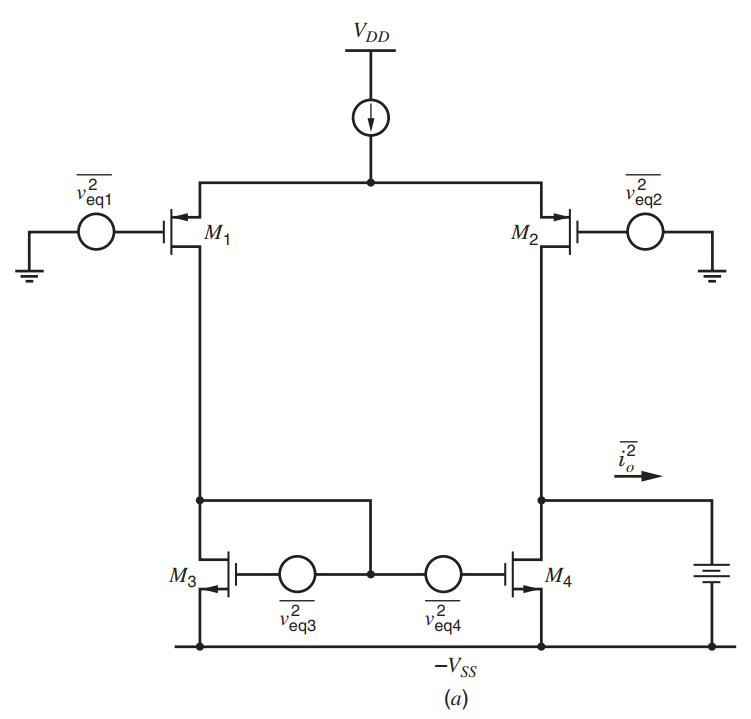
\includegraphics[width = 6.5cm]{DiffAmp_noise_1}
    \caption{สัญญาณรบกวนของทรานซิสเตอร์แต่ละตัวใน Differential Amplifier \cite{Grey09}}
    \label{DiffAmp_noise_1}
\end{figure}

\begin{figure}[h]
    \centering
    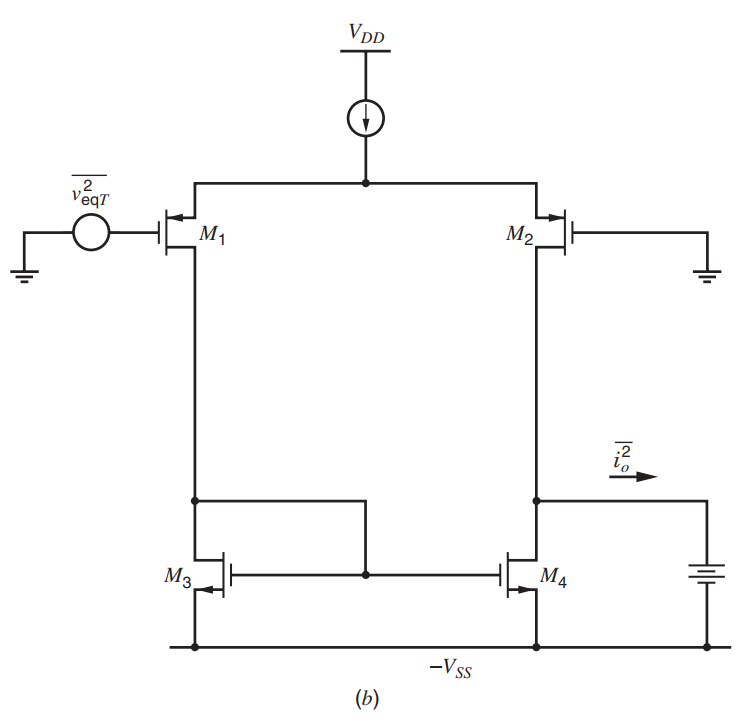
\includegraphics[width = 6.5cm]{DiffAmp_noise_2}
    \caption{วงจรสมมูลของสัญญาณรบกวนใน Differential Amplifier โดยรวมให้อยู่ในแหล่งจ่ายเดียว \cite{Grey09}}
    \label{DiffAmp_noise_2}
\end{figure}

จากรูปที่~\ref{DiffAmp_noise_1} สัญญาณรบกวนจากทรานซิสเตอร์ตัวต่าง ๆ ใน Differential Amplifier สามารถนำมารวมกันให้อยู่ในแหล่งจากแรงดันแหล่งเดียวได้ดังในรูปที่~\ref{DiffAmp_noise_2} โดยมีสมการดังนี้ คือ \cite{Grey09}
\begin{equation}
    \bar{v_{eqT}^2} = \bar{v_{eq1}^2} + \bar{v_{eq2}^2} + (g_{m3}/g_{m1})^2 (\bar{v_{eq3}^2} + \bar{v_{eq4}^2}) \label{Eq_DiffAmp_Lumped}
\end{equation}

จากสัญญาณรบกวนอ้างอิงขาเข้าของ MOSFET (สมการที่~\ref{Eq_MOS_noise})  นำสัญญาณรบกวนแบบ flicker noise ไปแทนในสมการที่~\ref{Eq_DiffAmp_Lumped} เพื่อให้ได้สัญญาณรบกวน flicker noise สมมูลแบบแหล่งจ่ายแรงดันแหล่งเดียว คือ
\begin{equation}
    \bar{v_{1/f}^2} = \frac{2K_p}{fW_1L_1C_{ox}}(1 + \frac{K_n\mu_nL_1^2}{K_p\mu_pL_3^2})\Delta f
    \label{Eq_DiffAmp_flicker}
\end{equation}

โดยที่ $K_p$ และ $K_n$ คือ flicker noise constant ของ PMOS และ NMOS ตามลำดับ

เช่นเดียวกันคือ จากสัญญาณรบกวนอ้างอิงขาเข้าของ MOSFET (สมการที่~\ref{Eq_MOS_noise})  นำสัญญาณรบกวนแบบ thermal noise ไปแทนในสมการที่~\ref{Eq_DiffAmp_Lumped} เพื่อให้ได้สัญญาณรบกวน thermal noise สมมูลแบบแหล่งจ่ายแรงดันแหล่งเดียว คือ
\begin{equation}
    \bar{v_{1/f}^2} = 4kT\frac{4}{3\sqrt{2\mu_pC_{ox}(W/L)_1I_D}}(1+\sqrt
    {\frac{\mu_n(W/L)_3}{\mu_p(W/L)_1}})\Delta f
    \label{Eq_DiffAmp_thermal}
\end{equation}

จากสมการที่~\ref{Eq_DiffAmp_flicker} การเพิ่ม W และ L ของทรานซิสเตอร์ $Q_1$ และ $Q_2$ จะทำให้สัญญาณรบกวนลดลงได้ แต่จะทำให้ความจุไฟฟ้าแบบต่าง ๆ ใน MOS เพิ่มขึ้น และทำให้ผลตอบสนองเชิงความถี่ของวงจร op amp นี้มี crossover frequency ที่ต่ำลง

ในขณะที่จากสมการที่~\ref{Eq_DiffAmp_thermal} การเพิ่มอัตราส่วน $W/L$ ของทรานซิสเตอร์ $Q_1$ และ $Q_2$ สามารถลดขนาดของสัญญาณรบกวนในวงจรได้เช่นกัน นอกจากนั้นการเพิ่มกระแสไบแอสในทรานซิสเตอร์ก็สามารถทำให้ลดสัญญาณรบกวนได้ แต่จะทำให้ช่วงสัญญาณขาเข้า (input common-mode range) และช่วงสัญญาณขาออก (output swing) มีค่าต่ำลงเนื่องจาก overdrive voltage ของทรานซิสเตอร์เพิ่มขึ้น นอกจากนั้นยังทำให้วงจรใช้พลังงานมากขึ้นด้วย

การต่อ body ของทรานซิสเตอร์ต่าง ๆ เข้าไปที่ขาของ power supply โดยตรงจะทำให้สัญญาณรบกวนของวงจร op amp ต่ำลงอย่างมีนัยสำคัญ

\subsubsection{Total Harmonic Distortion}

การคำนวณ Total Harmonic Distortion หรือ THD สามารถทำได้โดยการนำขนาดของ amplitude ของสัญญาณที่มี Harmonic สูงขึ้นไปเป็น 2,3,4,... เท่า เปรียบเทียบกับสัญญาณที่มี Harmonic พื้นฐานที่ต้องการจากวงจร ซึ่งใช้สมการดังนี้ในการคำนวณ
\begin{equation}
    THD = \frac{\sqrt{V_2^2 + V_3^2 + V_4^2 + ...}}{V_1}
\end{equation}

ในโปรแกรม LTSpice นั้น การคำนวณ Total Harmonic Distortion สามารถทำได้โดยใช้คำสั่ง \lstinline{.four} โดยสำหรับค่าเริ่มต้นในโปรแกรม จำนวน Harmonic ทั้งหมดที่โปรแกรมจะรวมให้ในการคำนวณ THD คือ 10 Harmonics

\subsubsection{แหล่งจ่ายกระแสอ้างอิง}

สำหรับแหล่งจ่ายกระแสอ้างอิง สามารถออกแบบเพื่อให้กระแสไม่เปลี่ยนแปลงไปเมื่อแรงดันจาก power supply เปลี่ยนแปลง การออกแบบดังกล่าวสามารถมีรูปแบบได้ดังรูปที่~\ref{bias_circuit}

\begin{figure}[h]
    \centering
    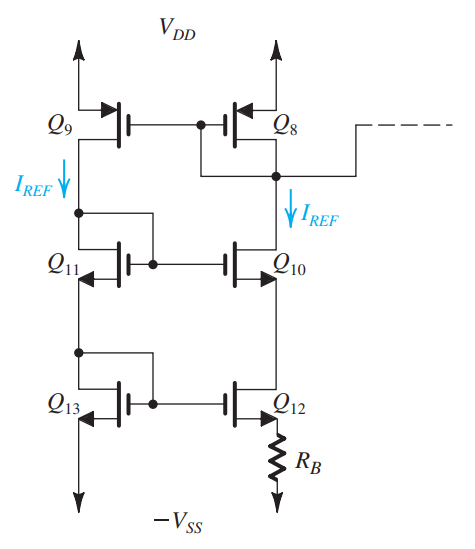
\includegraphics[width = 8cm]{bias_circuit}
    \caption{แหล่งจากอ้างอิงสำหรับ CMOS op amp โดยที่ $Q_8$ เป็นทรานซิสเตอร์ตัวเดียวกันกับ $Q_8$ ในวงจรของรูปที่~\ref{opamp-twostage} (จาก Sedra and Smith, Microelectronic Circuits, 7E \cite{Sedra15})}
    \label{bias_circuit}
\end{figure}

จากภาพ จะเห็นได้ว่า Q11 และ Q10 จะเป็น current mirror ให้กันและกัน นอกจากนั้น Q9 และ Q8 ต่างก็เป็น current mirror ซึ่งกันและกันเช่นกัน นั่นแสดงว่ากระแสไฟฟ้าในรางซ้ายจะถูกอ้างอิงกับกระแสไฟฟ้าในรางขวาเสมอ โดยขนาดของกระแสนั้นสามารถถูกกำหนดได้โดย Q13 และ Q12 ที่มีอัตราส่วนของ W/L ไม่เท่ากัน และมีตัวต้านทาน $R_B$ เพื่อเพิ่มข้อจำกัดของกระแสอ้างอิงนั้น

จากการคำนวณของ Sedra and Smith \cite{Sedra15} จะได้ว่าขนาดของ $R_B$ ในวงจรรูปที่~\ref{bias_circuit} สามารถออกแบบให้ได้ $I_{REF}$ ตามต้องการ โดยใช้สมการ
\begin{equation}
    R_B = \frac{2}{\sqrt{2\mu_nC_{ox}(W/L)_{12}I_{REF}}}(\sqrt{\frac{(W/L)_{12}}{(W/L)_{13}}} - 1)
    \label{bias_resistor}
\end{equation}

ซึ่งจะเห็นได้ว่าขนาดของ $I_{REF}$ เป็นอิสระจากแรงดันของ power supply และขนาดของ threshold voltage ของทรานซิสเตอร์ต่าง ๆ ในวงจร

\subsection{เงื่อนไขของการออกแบบวงจร}

สำหรับเงื่อนไข (specifications) ของวงจร op amp ซึ่งเป็นโจทย์ที่ทางบริษัทให้มา มีรายละเอียดดังนี้

\begin{enumerate}
    \item ออกแบบวงจร two-stage op amp โดยใช้เทคโนโลยี CMOS 0.18 nm ซึ่งมีโมเดลของ BSIM3 ให้มา
    \item Supply Voltage ของ op amp นี้จะมีค่าอยู่ระหว่าง 1.1 V ถึง 1.8 V (single supply)
    \item วงจร op amp ดังกล่าวต้องขับโหลดซึ่งเป็นตัวเก็บประจุขนาด $C_L$ = 100 \si{\femto F}
    \item การใช้พลังงานของวงจรจะต้องไม่เกิน 6 \si{\micro W}
    \item DC open-loop gain $\geq$ 60 dB
    \item ช่วงของสัญญาณขาออก (Output swing) $\geq$ $V_{DD}$ – 0.2 V \\(โดยที่ DC open-loop gain $\geq$ 60 dB)
    \item ช่วงของสัญญาณขาเข้า (Input common-mode voltage range) $\geq$ 50\% ของช่วง ($V_{DD} - V_{SS}$) \\(โดยที่ DC open-loop gain $\geq$ 60 dB)
    \item สัญญาณรบกวนอ้างอิงขาเข้ารวมของวงจร ตั้งแต่ความถี่ 1 Hz จนถึง 1 GHz เมื่อต่อวงจร op amp เป็นรูปแบบ unity-gain feedback ต้องมีค่าไม่เกิน 220 \textmu Vrms
    \item 1\% settling time ของผลตอบสนองแบบ step input ขนาด 0.5 V ต้องมีค่าไม่เกิน 2 \si{\micro s} เมื่อต่อวงจร op amp เป็นรูปแบบ unity-gain feedback
    \item total harmonic distortion ของสัญญาณขาออกเมื่อมีขนาดแบบขึ้นสุด ลงสุด จะต้องมีค่าไม่เกิน 0.2\%
    \item เนื่องจากการผลิตวงจร IC อาจมีความเบี่ยงเบนของค่า parameters ต่าง ๆ ของทรานซิสเตอร์จำนวนมากในวงจร ดังนั้นการจำลองวงจรควรที่จะคำนึงถึงค่า parameters ของทรานซิสเตอร์ต่าง ๆ ในกรณีที่มีโอกาสเบี่ยงเบนไปมากที่สุด ซึ่งเรียกโมเดลของทรานซิสเตอร์ที่มีค่าเบี่ยงเบนของ parameters ต่าง ๆ อย่างสุดขอบว่าเป็น process corner โดยสำหรับในการออกแบบวงจร op amp นี้ ให้ทดสอบในโมเดลแบบ TT, FF และ SS (ตัวอักษร T, F, S ย่อมาจาก typical, fast และ slow ตามลำดับ โดยตัวอักษรตัวแรกแทน process corner ของ NMOS และตัวอักษรตัวที่สองแทน process corner ของ NMOS)
    \item ในการจำลองวงจรในหัวข้อต่าง ๆ ให้จำลองในช่วงอุณหภูมิที่แตกต่างกันกันด้วย คือช่วงอุณหภูมิตั้งแต่  0\degree C. ถึง 70\degree C.
\end{enumerate}

\subsection{การออกแบบวงจรตามเงื่อนไข}

\subsubsection{การจำลองเพื่อหาคุณลักษณะของโมเดล CMOS}

ก่อนที่จะเริ่มออกแบบวงจร op amp ตามเงื่อนไขของโจทย์ ควรที่จะหา characteristics โดยคร่าวของโมเดล CMOS ก่อน ซึ่งได้แก่ threshold voltage, $k_{n}'$ หรือ $k_{p}'$ และ Early voltage $|V_A'|$

สำหรับโมเดล NMOS:
\begin{itemize}
    \item Threshold Voltage $|V_{tn}|$: 0.391 V
    \item $k_{n}'$: 392 \si{\micro A/V^2}
    \item $|V_A'|$: 20 \si{V/\micro m}
\end{itemize}

สำหรับโมเดล PMOS:
\begin{itemize}
    \item Threshold Voltage $|V_{tp}|$: 0.405 V
    \item $k_{p}'$: 89.0 \si{\micro A/V^2}
    \item $|V_A'|$: 28 \si{V/\micro m}
\end{itemize}

สำหรับ $V_{tn}$ และ $|V_{tp}|$ ถูกคำนวณในช่วง $|V_{gs}|$ ระหว่าง 0.39 V ถึง 0.70 V และ $|V_A'|$ ถูกคำนวณในช่วง $|V_{ds}|$ ระหว่าง 0.60 V ถึง 0.70 V โดยที่ $|V_A'|$ เป็นเพียงค่าประมาณเฉลี่ยเนื่องจากค่า $|V_A'|$ มีความไม่เป็นอิสระจาก $I_D$ ที่เปลี่ยนแปลงไปอีกด้วย

\subsubsection{โครงสร้างโดยคร่าวของ Op Amp}

\begin{figure}[h]
    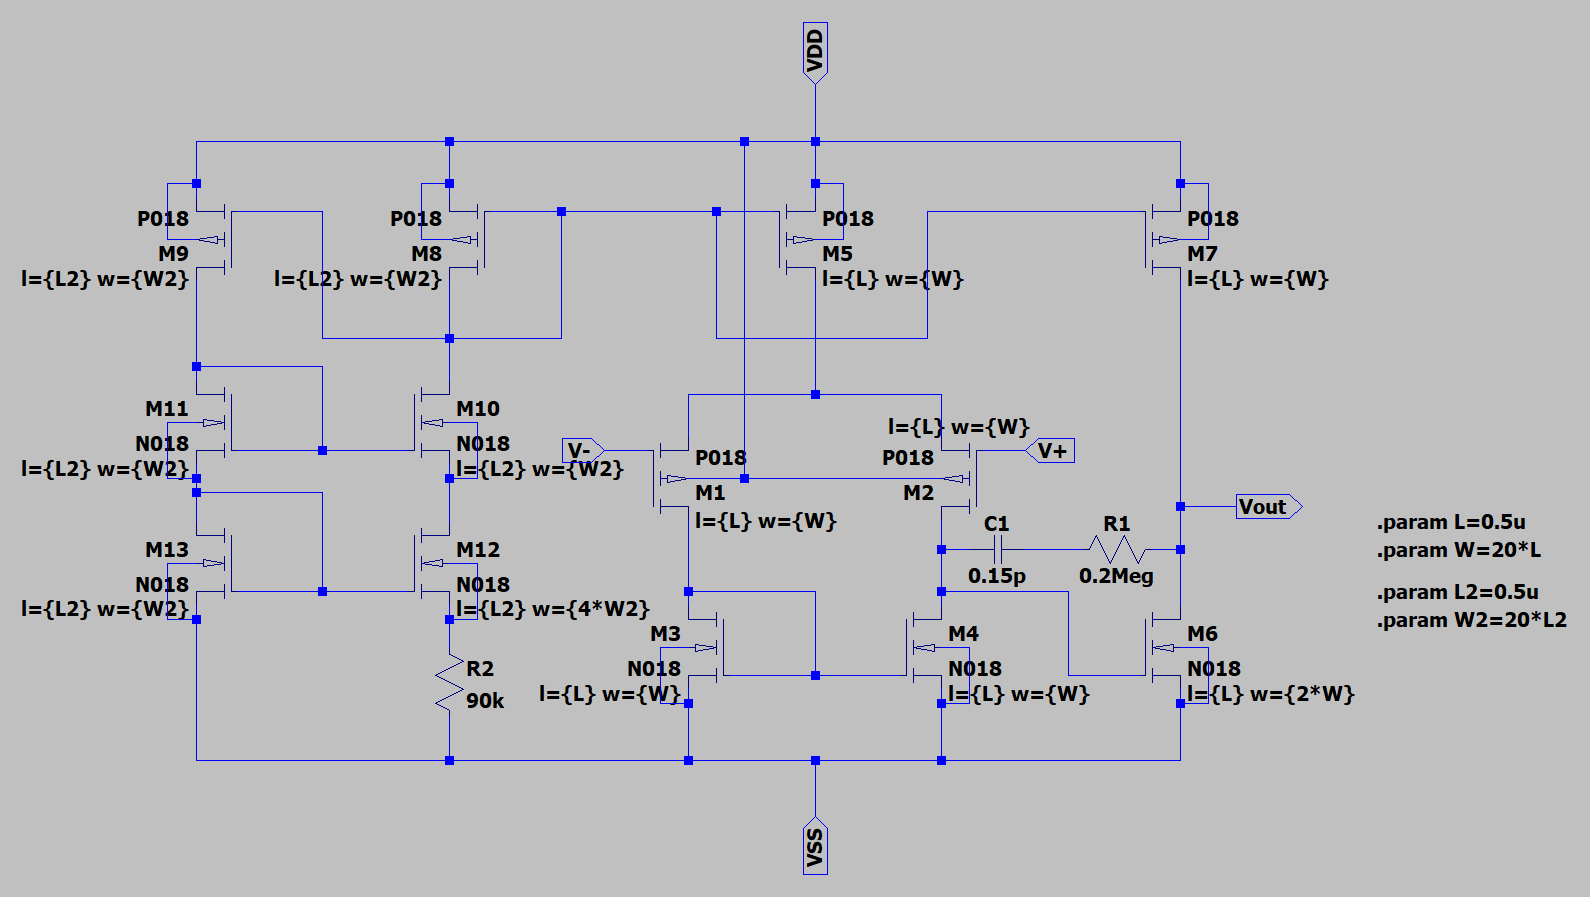
\includegraphics[width = \linewidth]{my_op_amp}
    \caption{วงจร op amp ของผู้จัดทำ}
    \label{my_op_amp}
\end{figure}

\subsubsection{การจัดการพลังงาน}

เนื่องจากวงจร op amp ที่ออกแบบไม่สามารถใช้พลังงานได้เกิน 6 \si{\micro W} และเนื่องจากแรงดันจาก power supply สามารถมีค่าได้มากที่สุดคือ 1.8 V จากสมการ $P = VI$ ได้ว่ากระแสที่จ่ายมาจาก power supply จะต้องมีค่าไม่เกิน 3.3 \si{\micro A}

จากรูปที่~\ref{my_op_amp} เนื่องจากมีรางของกระแสทั้งหมด 4 ราง ดังนั้น $I_{REF}$ จึงควรมีค่าไม่เกิน $3.3/4 = 0.83$ \si{\micro A} ดังนั้น เพื่อความเผื่อเกิน จึงจะออกแบบวงจรเพื่อให้ $I_{REF}$ มีค่าเป็น 0.5 \si{\micro A}

\subsubsection{การออบแบบวงจรไบแอสกระแสอ้างอิง}

จากสมการที่~\ref{bias_resistor} เมื่อให้ $\frac{(W/L)_{12}}{(W/L)_{13}} = 4$ โดยที่ $(W/L)_{13}$ เท่ากับ 20, $I_{REF} = \num{0.5e-6}$, $k_{n}' = \num{392e-6}$ ค่าของ $R_B$ ที่คำนวณได้จะมีค่าเป็น 11.3 \si{\kilo\ohm}

ไม่ว่าอย่างไรก็ตาม ค่าของกระแส $I_{REF}$ กลับมีค่ามากกว่า 0.5 \si{\micro A} มาก เกินอะไรขึ้น?

\subsubsection{การจำลองเพื่อหาคุณลักษณะของโมเดล CMOS ตอนที่สอง}

ความผิดพลาดของการหาคุณลักษณะของโมเดล CMOS ในตอนแรกคือการหาคุณลักษณะในช่วงการทำงานที่ไม่ใช่ช่วงการทำงานที่ใช้จริง ดังนั้นจึงควรหาคุณลักษณะใหม่อีกครั้ง โดยเปลี่ยนช่วงการจำลองของ $|V_{gs}|$ เป็นช่วง 0.20 V ถึง 0.36 V สำหรับ NMOS และ 0.25 V ถึง 0.45 V สำหรับ PMOS (ซึ่งเป็นช่วงที่ค่ากระแส $I_D = \num{0.5e-6}$) ผลลัพธ์ของคุณลักษณะของโมเดล CMOS จะเปลี่ยนเป็น

สำหรับโมเดล NMOS:
\begin{itemize}
    \item Threshold Voltage: 0.235 V
    \item $k_{n}'$: 19.7 \si{\micro A/V^2}
\end{itemize}

สำหรับโมเดล PMOS:
\begin{itemize}
    \item Threshold Voltage: 0.299 V
    \item $k_{p}'$: 15.2 \si{\micro A/V^2}
\end{itemize}

เนื่องจากช่วงการทำงานที่ใช้จริง กระแส $I_D$ มีค่าต่ำมาก ๆ จนได้ว่า CMOS จะทำงานอยู่ในช่วงของ subthreshold

\subsubsection{การออบแบบวงจรไบแอสกระแสอ้างอิง ตอนที่สอง}

จากคุณลักษณะของโมเดล CMOS ที่หาได้ใหม่จากหัวข้อที่แล้ว จะได้ว่า $R_B$ ที่คำนวณได้ใหม่จะมีค่าเป็น 50.4 \si{\kilo\ohm} ไม่ว่าอย่างไรก็ตาม ค่าของ $I_{REF}$ ที่จำลองได้จริงก็ยังคงมีค่ามากกว่าที่ต้องการอยู่ การปรับละเอียด (fine-tuning) จึงยังคงจำเป็น และได้ว่าค่า $R_B$ ที่ต้องการในตอนสุดท้าย คือ 90 \si{\kilo\ohm} ซึ่งทำให้ได้กระแสงอ้างอิง $I_{REF}$ ที่มีค่าเป็น 0.657 \si{\micro A}\footnote{โดยใช้โมเดลแบบ TT CMOS และจำลองที่อุณหภูมิ 35\si{\degreeCelsius}}

ค่าของ $R_B$ ไม่ควรสูงเกินไปเนื่องจากจะทำให้พื้นที่ที่ใช้ในวงจรรวมเพิ่มขึ้น

\subsubsection{การออกแบบวงจรขยายทั้งสอง stage}

เมื่อเลือกอัตราส่วนของ $W/L$ ของ MOS ทุกตัวเป็น 20 (ยกเว้น $Q_6$ ที่จะต้องมีค่า $W/L$ เท่ากับ 40 เนื่องด้วยสมการที่~\ref{offset-eq}.) และให้ L ของ MOS ทุกตัวเป็น 0.5 \si{\micro m}

เมื่อใช้สมการที่~\ref{gain-1} และสมการที่~\ref{gain-2} แทนค่าคุณลักษณะต่าง ๆ ของ CMOS ที่เกี่ยวข้องทั้งหมดเข้าไปในสมการ จะได้ค่าของ $A_1 = A_2 = 571$ ดังนั้น DC open-loop gain ของวงจรที่ออกแบบได้ในเชิงทฤษฎีจะมีค่าเป็น $A_1A_2 = \num{8.16e4}$ = 98.2 dB 

สำหรับในการจำลองวงจร ได้ว่าค่าของ DC open-loop gain จะมีค่าเพียงประมาณ 80 dB แต่ก็ยังเกินจากเงื่อนไขที่กำหนดไว้ในโจทย์

ค่าของ DC open-loop gain สามารถทำให้สูงขึ้นได้หากเพิ่มความยาว L ของ MOS แต่ crossover frequency ของผลตอบสนองเชิงความถี่จะลดลงเนื่องจาก $\omega_{P2}$ ที่ลดลง. นอกจากนั้นการลด $I_D$ จะสามารถเพิ่ม DC open-loop gain ได้ แต่ขนาดของสัญญาณรบกวนอ้างอิงขาเข้าก็จะเพิ่มขึ้นตามไป

\subsubsection{การออกแบบผลตอบสนองเชิงความถี่ของอัตราขยายแบบวงเปิด (open-loop gain) ของวงจร}

จากตำแหน่งของ dominant pole $\omega_{P1}$ ในสมการที่~\ref{pole-zero-approx} และขนาดของ DC open-loop gain ในสมการที่~\ref{gain-1} และสมการที่~\ref{gain-2} เราสามารถคำนวณหาตำแหน่งของ crossover frequency ได้เป็น 

$$\omega_t = G_{m1}/C_C$$

โดยค่าของ $G_{m1}$ สามารถคำนวณได้จาก $g_{m} = \sqrt{2k_n'(W/L)I_D}$ และถ้าหากเลือกค่า $C_C$ = 0.15 pF, จะได้ว่าค่าของ crossover frequency หรือ $\omega_t$ จะมีค่าเป็น 17.1 MHz.

จากการจำลองวงจร ได้ว่า $\omega_t$ อยู่ในช่วงระหว่าง 9 ถึง 13 MHz ซึ่งยังเกินจากเงื่อนไขที่กำหนดไว้ในโจทย์

การออกแบบ crossover frequency $\omega_t$ ไม่ควรจะมีค่ามากกว่านี้อีก เนื่องจากขนาดของ phase margin จะมีค่าลดลงมากเนื่องจากตำแหน่งของขั้วที่สอง: $\omega_{P2}$. 

ปัญหาที่แก้ได้ยากของการออกแบบผลตอบสนองเชิงความถี่ของอัตราขยายแบบวงเปิด เกิดจากตำแหน่งของขั้วที่สอง, $\omega_{P2}$, ซึ่งมีค่าเป็น $\omega_{P2} = G_{m2}/C_2$ เนื่องจาก $C_2$ เป็นค่าที่กำหนดมาจาก $C_L$ และความจุไฟฟ้าตามคุณลักษณะของ MOS ตัวต่าง ๆ และค่าของ $G_{m2}$ ก็สามารถเปลี่ยนได้ยากเนื่องจากการเปลี่ยนค่าดังกล่าวจะทำให้ค่าคุณลักษณะของวงจร op amp ที่ออกแบบไว้แล้วเปลี่ยนแปลงไปด้วย ดังนั้น ขั้วที่สองดังกล่างจึงดูเหมือนว่าถูกกำหนดไว้แล้วและเปลี่ยนแปลงได้ยาก ซึ่งหากเราต้องการเพิ่ม phase margin ของผลตอบสนองดังกล่าว เราจะต้องออกแบบ crossover frequency หรือ $\omega_t$ ให้ต่ำพอ โดยอาจต่ำกว่าค่าของ $\omega_{P2}$ ประมาณ 1 decade ลงไป ไม่ว่าอย่างไรก็ตามการทำเช่นนั้นจะทำให้ค่าของ crossover frequency ต่ำเกินไป

ค่าของ $\omega_{P2}$ สามารถคำนวณได้ยากเนื่องจากขึ้นอยู่กับ $C_2$ ที่ประกอบด้วยความจุไฟฟ้าตามคุณลักษณะของ MOS ตัวต่าง ๆ ดังนั้นการนำค่าจากผลการจำลองมาใช้เลยน่าจะเป็นทางเลือกที่ดีกว่า ซึ่งการประมาณค่าของ $\omega_{P2}$ (โดยใช้การลากเส้นโดยคร่าวบนรูปที่~\ref{openloopgain_freqresponse}) สามารถหาได้ว่าอยู่ที่ประมาณ 20 MHz.

การแก้ปัญหาที่เกิดจาก $\omega_{P2}$ ได้กล่าวไว้แล้วในสมการที่~\ref{new-zero} โดยการออกแบบวงจรจะต้องต่อ $R$ อนุกรมกับ $C_C$ เพื่อเปลี่ยนตำแหน่งของ zero ให้อยู่ที่ left complex plane แทน โดยหากเลือกค่าของ $\omega_{Z}$ อย่างระมัดระวัง ให้มีค่าอยู่ต่ำกว่าตำแหน่งของ $\omega_{P2}$ เล็กน้อย จทำให้ขั้ว $\omega_{P2}$ ดังกล่าวถูกยกเลิก (cancelled) ไป 

โดยจากสมการ~\ref{new-zero} เมื่อเลือกค่า R = 200 \si{\kilo\ohm} จะทำให้ได้ค่าของ $\omega_{Z}$ อยู่ที่ประมาณ 6.2 MHz ซึ่งตรงกับผลการจำลองของวงจรในโปรแกรม

Phase margin ของ open-loop gain จากการคำนวณควรจะมีค่าน้อยกว่า 90 องศาเล็กน้อย เนื่องจากขั้วแรกและขั้วที่สองที่อยู่ใกล้กับ crossover frequency

\subsubsection{Slew Rate}

จากเงื่อนไขของการออกแบบในโจทย์ ค่าของสัญญาณขาออกจะต้องตาม 0.5-V step input ในเวลาไม่เกิน 2 \si{\micro s} ดังนั้น slew rate ของสัญญาณขาออกจะต้องมีค่าไม่ต่ำกว่า $0.5/\num{2e-6} = \num{2.5e5}$ V/s.

จากสมการที่~\ref{slew-eq} การคำนวณ slew rate ได้ค่าออกมาเป็น \num{2.19e6} V/s ซึ่งมีค่ามากกว่าที่โจทย์ได้กำหนดเอาไว้มาก

\subsubsection{การออกแบบเพื่อลดสัญญาณรบกวน}

เนื่องจากการคำนวณสัญญาณรบกวนของวงจรค่อนข้างมีความซับซ้อนมาก การจำลองวงจรน่าจะทำให้การออกแบบเป็นไปได้ง่ายกว่า

การลดสัญญาณรบกวนของวงจรมีวิธีทั่วไปสองแบบ คือการเพิ่มอัตราส่วน W/L ของทรานซิสเตอร์ที่เกี่ยวข้องกับการขยายสัญญาณ และการต่อ body ของทรานซิสเตอร์เข้าไปที่แหล่ง power supply โดยตรง

\subsubsection{ช่วงของสัญญาณขาเข้า (Input Common-Mode Range) และสัญญาณขาออก  (Output Swing)}

ขนาดของ overdrive voltage ของแต่ละทรานซิสเตอร์สามารถคำนวณได้จาก
$$\frac{1}{2}k_n'(W/L)V_{ov}^2 = I_D$$

จากสมการดังกล่าวจะได้ว่า $|V_{ov6}| = |V_{ov3}| = 0.041 \si{V}$, $|V_{ov5}| = |V_{ov7}| = 0.066 \si{V}$, and $|V_{ov1}| = 0.046 \si{V}$.

โดยเมื่อพิจารณาร่วมกับข้อมูล $|V_{tn}|$ และ $|V_{tp}|$ และจากสมการที่~\ref{input-range} จะได้ว่า

\begin{itemize}
    \item ช่วงของสัญญาณขาเข้า (input common-mode range) คือตั้งแต่ -0.023 V ถึง $v_{DD}$ - 0.411 V
    \item ช่วงของสัญญาณขาออก (output swing) คือตั้งแต่ 0.041 V ถึง $v_{DD}$ - 0.066 V
\end{itemize}

ยิ่งช่วงของสัญญาณขาออก (output swing) มีความกว้างมากขึ้นเท่าไหร่ ขนาดของ total-harmonic-distortion (THD) ของสัญญาณขาออกก็จะยิ่งลดลงเท่านั้น

\subsection{การจำลองวงจรและผลการทดลอง}
\label{result-1}

\subsubsection{ผลตอบสนองเชิงความถี่ของอัตราขยายแบบวงเปิด: DC Gain, Crossover Frequency และ Phase Margin}

\begin{figure}
    \centering
    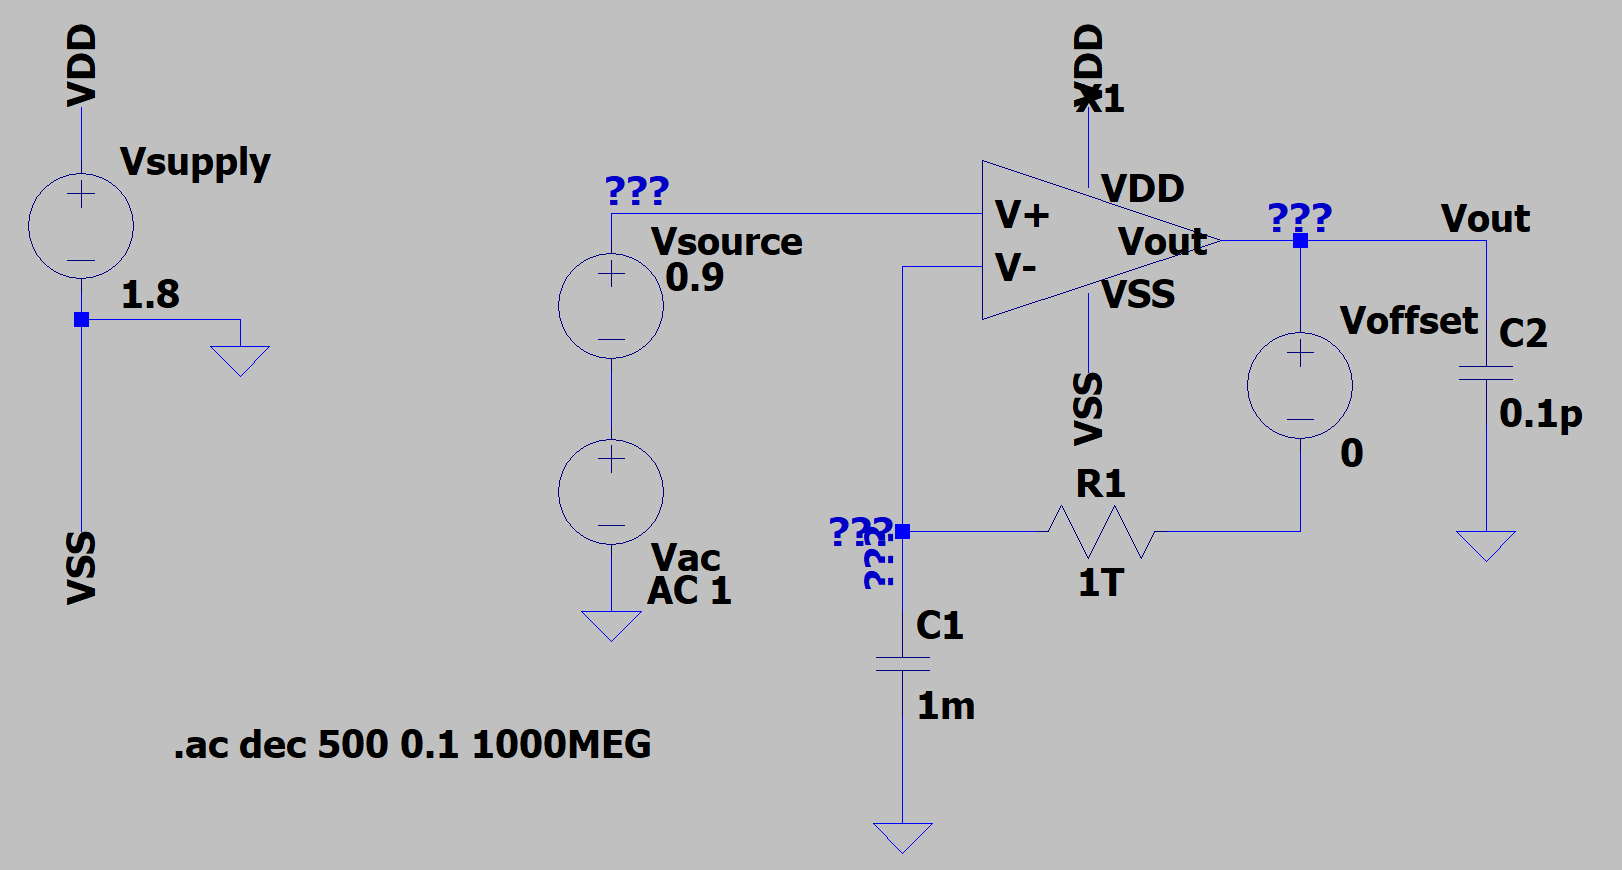
\includegraphics[width = 10cm]{measure-openloopgain}
    \caption{วงจรเพื่อจำลองผลตอบสนองเชิงความถี่ของอัตราขยายแบบวงเปิด}
    \label{measure-openloopgain}
\end{figure}

\paragraph{สำหรับการจำลองของตอนนี้จะมีทั้งหมด 171 การทดลอง ดังนี้}

\begin{itemize}
    \item ทดสอบบน 3 process corners (FF, TT, SS).
    \item แต่ละ process corner ใช้แรงดันของแหล่งจ่ายเป็น 1.1 V และ 1.8 V
    \item กรณีที่เป็น 1.1 V:
    \begin{itemize}
        \item เปลี่ยนค่าของแรงดันขาเข้า: 0.1, 0.3, 0.5, 0.7, 0.9 V
        \item เปลี่ยนค่าของแรงดันขาออก: 0.1, 0.55, 1.0 V
    \end{itemize}
    \item กรณีที่เป็น 1.8 V:
    \begin{itemize}
        \item เปลี่ยนค่าของแรงดันขาเข้า: 0.1, 0.4, 0.7, 1.0, 1.3, 1.6 V
        \item เปลี่ยนค่าของแรงดันขาออก: 0.1, 0.5, 0.9, 1.3, 1.7 V
    \end{itemize}
    \item แต่ละการทดลอง ทำที่อุณหภูมิ 0, 35, 70 \si{\degreeCelsius}.
\end{itemize}

\paragraph{ผลการทดลองแบบสรุป}

\begin{itemize}
    \item ค่าของ DC gain $\geq$ 60 dB สำหรับทั้ง 171 การทดลอง
    \item ค่าของ Phase Margin $\geq$ 60 degrees สำหรับทั้ง 171 การทดลอง
    \item ค่าของ Crossover frequency $\geq$ 7 MHz สำหรับทั้ง 171 การทดลอง \textbf{ยกเว้น}ในการทดลองต่อไปนี้
    \begin{itemize}
        \item $V_{in}$ = 1.6 V เมื่อ $V_{supply}$ = 1.8 V.
        \item $V_{in}$ = 0.7 V และ 0.9 V เมื่อ $V_{supply}$ = 1.1 V.
    \end{itemize}
\end{itemize}

\subsubsection{การใช้พลังงาน}

\begin{figure}[h]
    \centering
    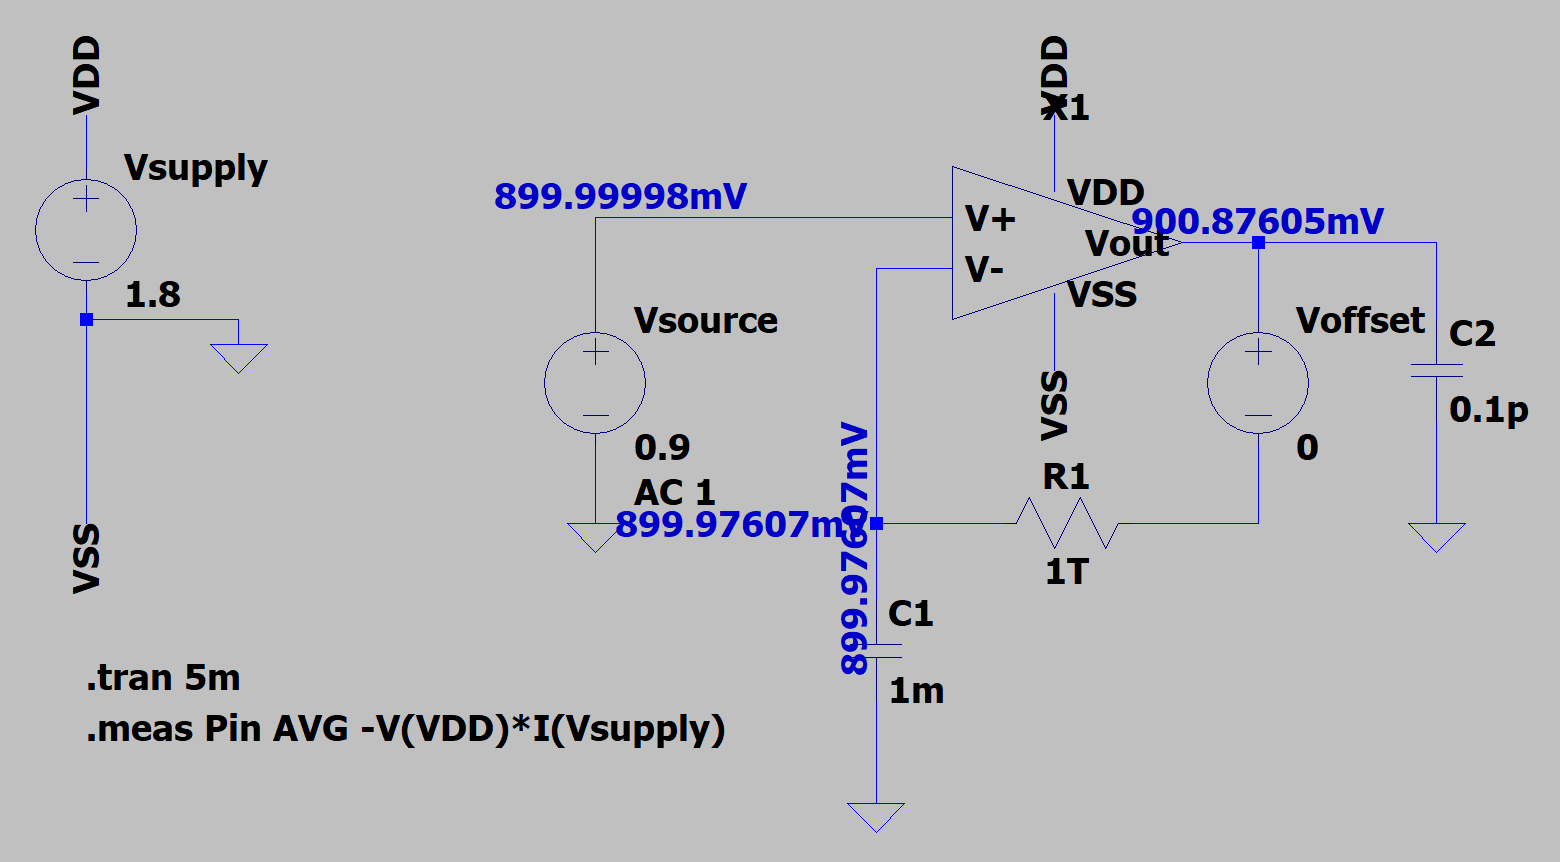
\includegraphics[width = 10cm]{measure-power}
    \caption{วงจรเพื่อทดสอบการใช้พลังงานของ op amp}
    \label{measure-power}
\end{figure}

การวัดการใช้พลังงานของวงจร op amp อย่างง่ายที่สุดคือการวัดค่าแรงดันและกระแสของแหล่งจ่ายไฟ แล้วนำมาคำนวณต่อเป็นกำลังไฟฟ้าอีกทีหนึ่ง

\paragraph{สำหรับการจำลองของตอนนี้จะมีทั้งหมด 18 การทดลอง ดังนี้}

\begin{itemize}
    \item ทดสอบบน 3 process corners (FF, TT, SS).
    \item แต่ละ process corner ใช้แรงดันของแหล่งจ่ายเป็น 1.1 V และ 1.8 V
    \item แต่ละการทดลอง ทำที่อุณหภูมิ 0, 35, 70 \si{\degreeCelsius}.
\end{itemize}

\paragraph{ผลการทดลองแบบสรุป}

\begin{itemize}
    \item สำหรับ power supply ค่าแรงดัน 1.8 V, \\ได้ว่า การใช้กำลังไฟฟ้าอยู่ในช่วง 4.11 ถึง 5.06 \si{\micro W}
    \item สำหรับ power supply ค่าแรงดัน 1.1 V, \\ได้ว่า การใช้กำลังไฟฟ้าอยู่ในช่วง 1.74 ถึง 2.22 \si{\micro W}
\end{itemize}

\subsubsection{การทดสอบสัญญาณรบกวน}

\begin{figure}[h]
    \centering
    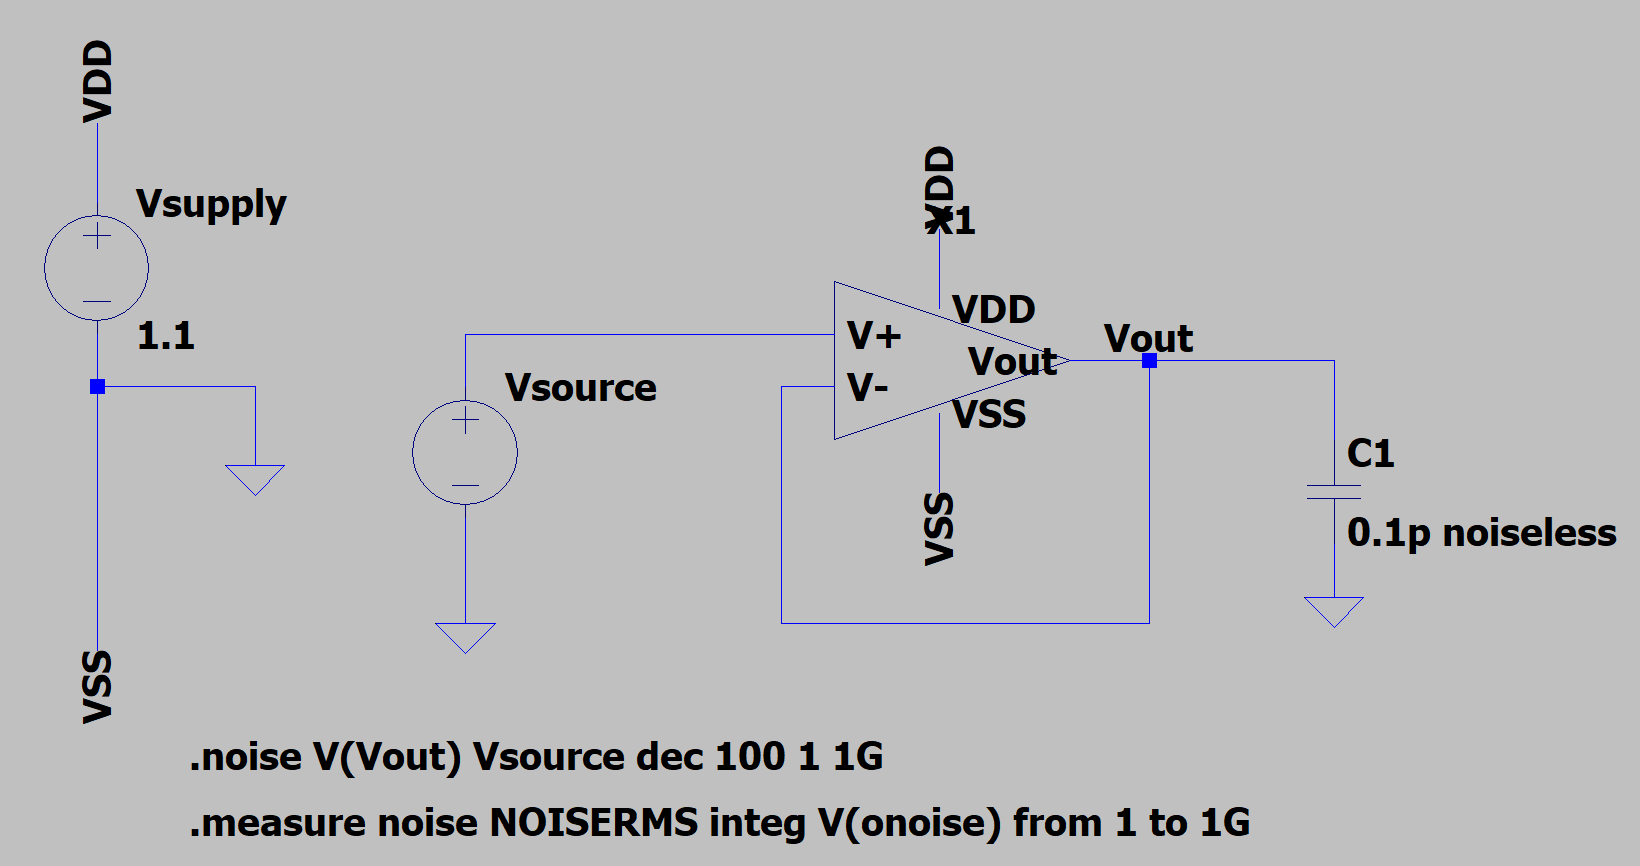
\includegraphics[width = 10cm]{measure-noise}
    \caption{วงจรที่ใช้สำหรับวัดค่าสัญญาณรบกวนอ้างอิงขาเข้า ซึ่งวัดจาก $V_{out}$.}
    \label{measure-noise}
\end{figure}

\paragraph{สำหรับการจำลองของตอนนี้จะมีทั้งหมด 18 การทดลอง ดังนี้}

\begin{itemize}
    \item ทดสอบบน 3 process corners (FF, TT, SS).
    \item แต่ละ process corner ใช้แรงดันของแหล่งจ่ายเป็น 1.1 V และ 1.8 V
    \item แต่ละการทดลอง ทำที่อุณหภูมิ 0, 35, 70 \si{\degreeCelsius}.
\end{itemize}

\paragraph{ผลการทดลองแบบสรุป}

ขนาดของสัญญาณรบกวนอ้างอิงขาเข้ารวมแบบ root-mean square รวมตั้งแต่ความที่ 1 Hz ถึง 1 GHz ในทุกการทดลอง มีค่าอยู่ในช่วง 120 to 180 \textmu Vrms.

\subsubsection{การทดสอบ Settling Time}

\begin{figure}[h]
    \centering
    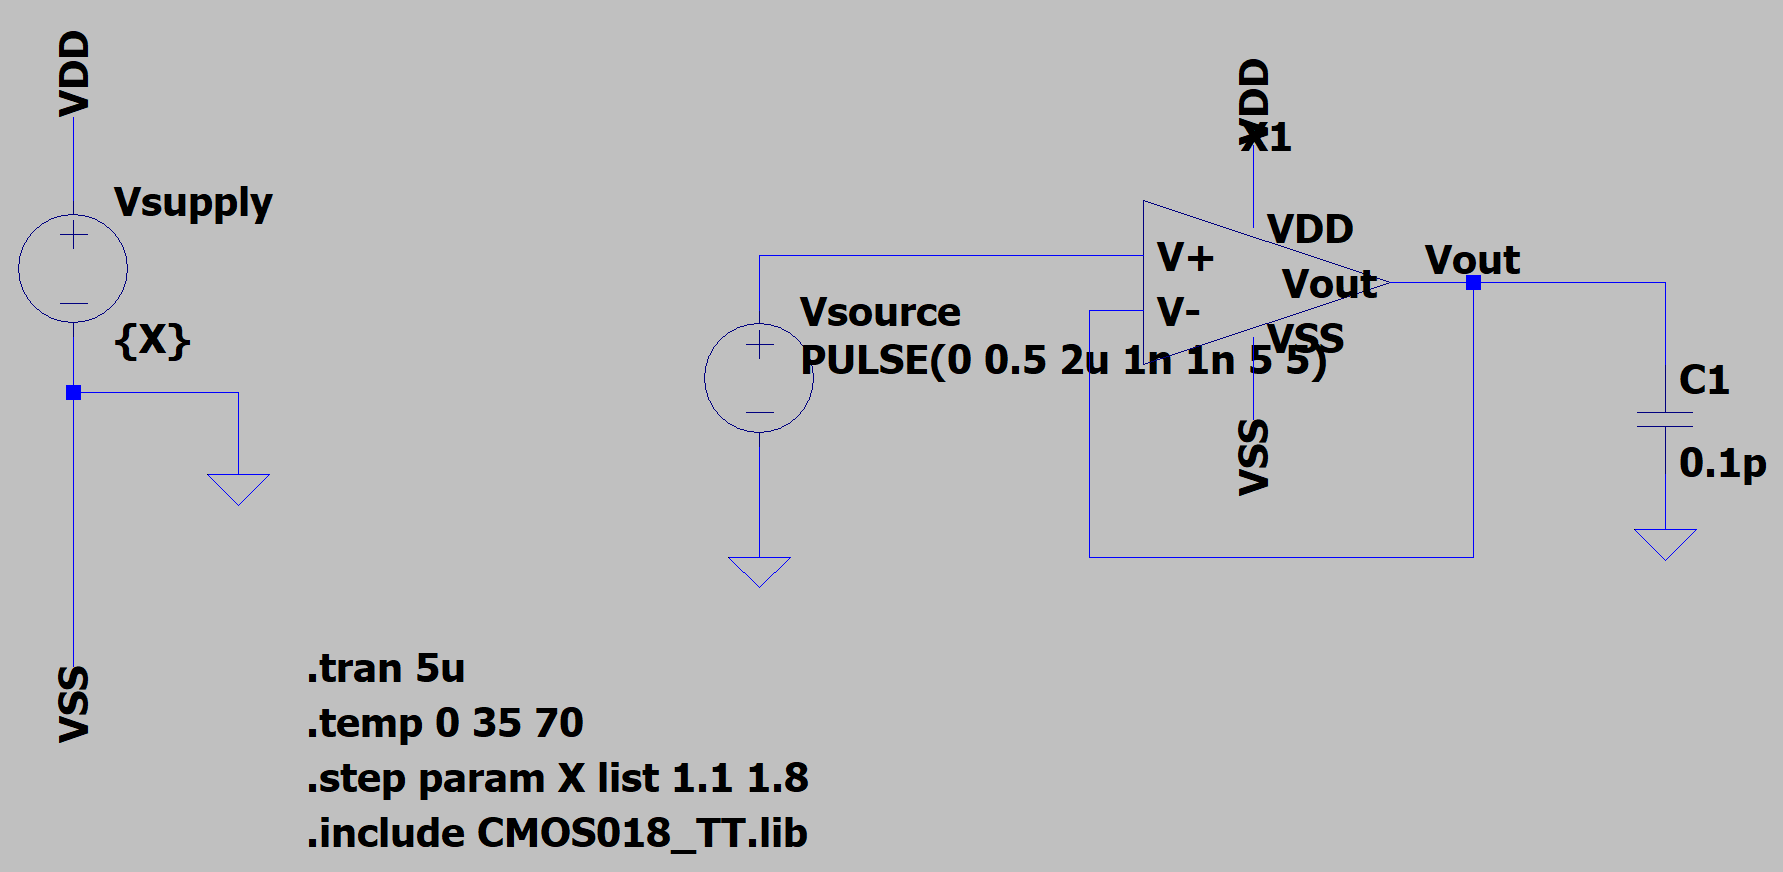
\includegraphics[width = 10cm]{measure-settlingtime}
    \caption{วงจรที่ใช้สำหรับวัด Settling Time}
    \label{measure-settlingtime}
\end{figure}

\paragraph{สำหรับการจำลองของตอนนี้จะมีทั้งหมด 18 การทดลอง ดังนี้}

\begin{itemize}
    \item ทดสอบบน 3 process corners (FF, TT, SS).
    \item แต่ละ process corner ใช้แรงดันของแหล่งจ่ายเป็น 1.1 V และ 1.8 V
    \item แต่ละการทดลอง ทำที่อุณหภูมิ 0, 35, 70 \si{\degreeCelsius}.
\end{itemize}

\paragraph{ผลการทดลองแบบสรุป}

ช่วงของ 1\% settling time ในทุกการทดลองอยู่ระหว่าง 0.35 ถึง 0.57 \si{\micro s}

\subsubsection{การทดสอบ Total Harmonic Distortion}

\begin{figure}[h]
    \centering
    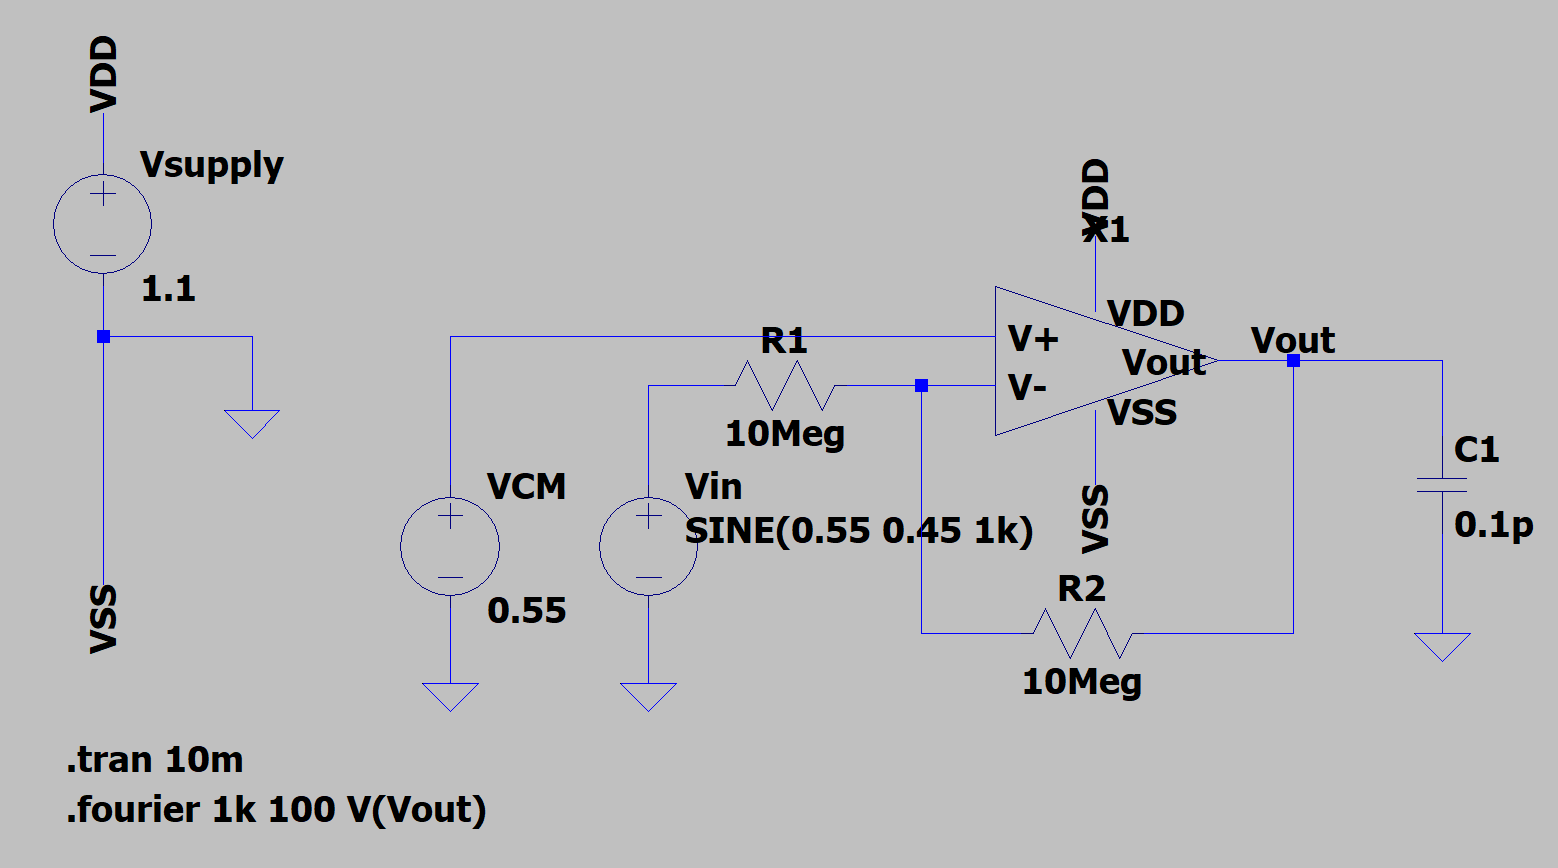
\includegraphics[width = 10cm]{measure-thd}
    \caption{วงจรที่ใช้สำหรับทดสอบ Settling Time}
    \label{measure-thd}
\end{figure}

THD วัดโดยใช้ output swing แบบ sine wave ที่ขึ้นสุดลงสุดในช่วง $V_{DD}$ - 0.2 V.

\paragraph{สำหรับการจำลองของตอนนี้จะมีทั้งหมด 18 การทดลอง ดังนี้}

\begin{itemize}
    \item ทดสอบบน 3 process corners (FF, TT, SS).
    \item แต่ละ process corner ใช้แรงดันของแหล่งจ่ายเป็น 1.1 V และ 1.8 V
    \item แต่ละการทดลอง ทำที่อุณหภูมิ 0, 35, 70 \si{\degreeCelsius}.
\end{itemize}

\paragraph{ผลการทดลองแบบสรุป}

ช่วงของ 1\% settling time ในทุกการทดลองอยู่ระหว่าง 0.35 ถึง 0.57 \si{\micro s}

\subsubsection{การเขียนโค้ดเพื่อให้สามารถรันการทดลองบน LTSpice แบบอัตโนมัติ}

\begin{itemize}
    \item ใช้ LTSpice ในการจำลองพฤติกรรมของวงจรไฟฟ้า
    \item การรันอัตโนมัติสั่งผ่านโค้ดของ Python
    \item ใช้ PyLTSpice Python library จาก Nuno Brum ซึ่งสามารถรันไฟล์ของ LTSpice ได้โดยตรง, สามารถเปลี่ยนค่าขององค์ประกอบในวงจร, อ่านไฟล์ \lstinline{.raw} ซึ่งมีผลของการจำลองวงจรได้จากโค้ดของ Python โดยตรง \cite{Brum22}
\end{itemize}

\subsection{การพัฒนาวงจรที่ออกแบบ}

เนื่องจากในวงจร op amp ที่ออกแบบในรูปที่~\ref{my_op_amp} ยังมีตัวต้านทานขนาดใหญ่ถึงสองตัว ซึ่งอาจจะทำให้วงจรกินพื้นที่ของ IC ค่อนข้างมาก จึงสามารถพัฒนาต่อได้อีก ดังนี้

\subsubsection{การแทนที่ตัวต้านทานที่ต่ออนุกรมกับ $C_C$ ด้วย transmission gate}

\begin{figure}[h]
    \centering
    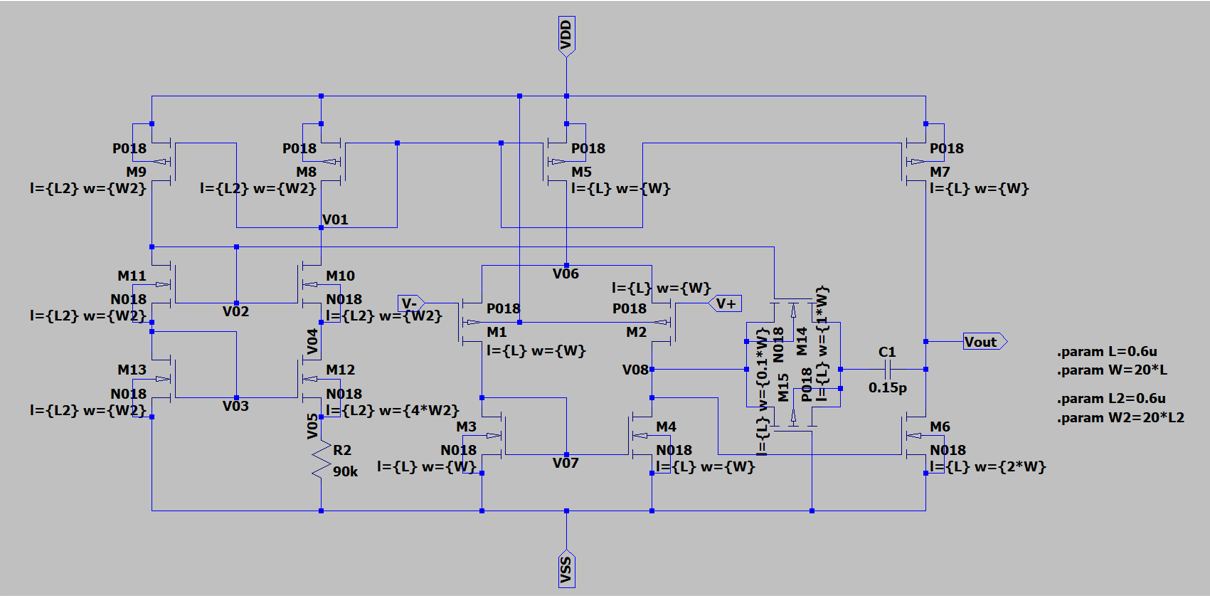
\includegraphics[width = \linewidth]{opamp-improve-1}
    \caption{การแทนที่ตัวต้านทานที่ต่ออนุกรมกับ $C_C$ ด้วย transmission gate}
    \label{opamp-improve-1}
\end{figure}

เนื่องจาก MOSFET สามารถทำหน้าที่เป็นตัวต้านทานได้เช่นกัน โดยการไบแอสแรงดันที่ขา gate ของทรานซิสเตอร์เพื่อให้ได้ช่วงในการทำงานอยู่ในช่วง triode region โดยเราสามารถไบแอสแรงดันได้โดยใช้วงจรสร้างกระแสที่ได้สร้างไว้แล้ว และเนื่องจากวงจรสร้างกระแสดังกล่าวสามารถให้แรงดันที่ค่อนข้างคงที่ ดังนั้นจึงได้ว่าแรงดันดังกล่าวมีความเหมาะสมที่จะใช้ในการไบแอสแรงดันที่ขา gate นั้น

สำหรับในรูปที่~\ref{opamp-improve-1} ตัว MOSFET ที่ทำหน้าที่ในการเป็นตัวต้านทานคือ Q14 และ Q15 โดยเหตุผลที่ใช้ทั้ง PMOS และ NMOS พร้อมกันเนื่องจากเพื่อทำให้การทำงานของ resistor นั้นกว้างขึ้น กล่าวคือ ไม่ถูก cutoff พร้อมกันทั้งสองทรานซิสเตอร์ \cite{Nath17}

สำหรับสมการของความต้านทานที่สร้างจาก PMOS และ NMOS ดังกล่าว สามารถเขียนได้ดังนี้ \cite{Nath17}
$$R = (\mu_n C_{ox} (W/L)_n (V_{GS}-V_{tn}) + \mu_p C_{ox} (W/L)_p (V_{SG}-|V_{tp}|))^{-1}$$

เราสามารถปรับอัตราส่วนของ $W/L$ ของทรานซิสเตอร์ Q14 และ Q15 แบบ fine-tuning จนกระทั่งได้ผลตอบสนองเชิงความถี่ของอัตราขยายวงเปิดที่ใกล้เคียงกับแบบเดิม 

สำหรับผลการทดลองที่ได้จากการจำลองวงจรในรูปที่~\ref{opamp-improve-1} เหมือนกับที่ได้จากวงจรในรูปที่~\ref{my_op_amp} ในทุกการทดลองที่ทำในหัวข้อที่~\ref{result-1}

\subsubsection{การเปลี่ยนวงจรสร้างกระแสอ้างอิงเพื่อให้มีขนาดของตัวต้านทานที่ลดลง}

\begin{figure}[h]
    \centering
    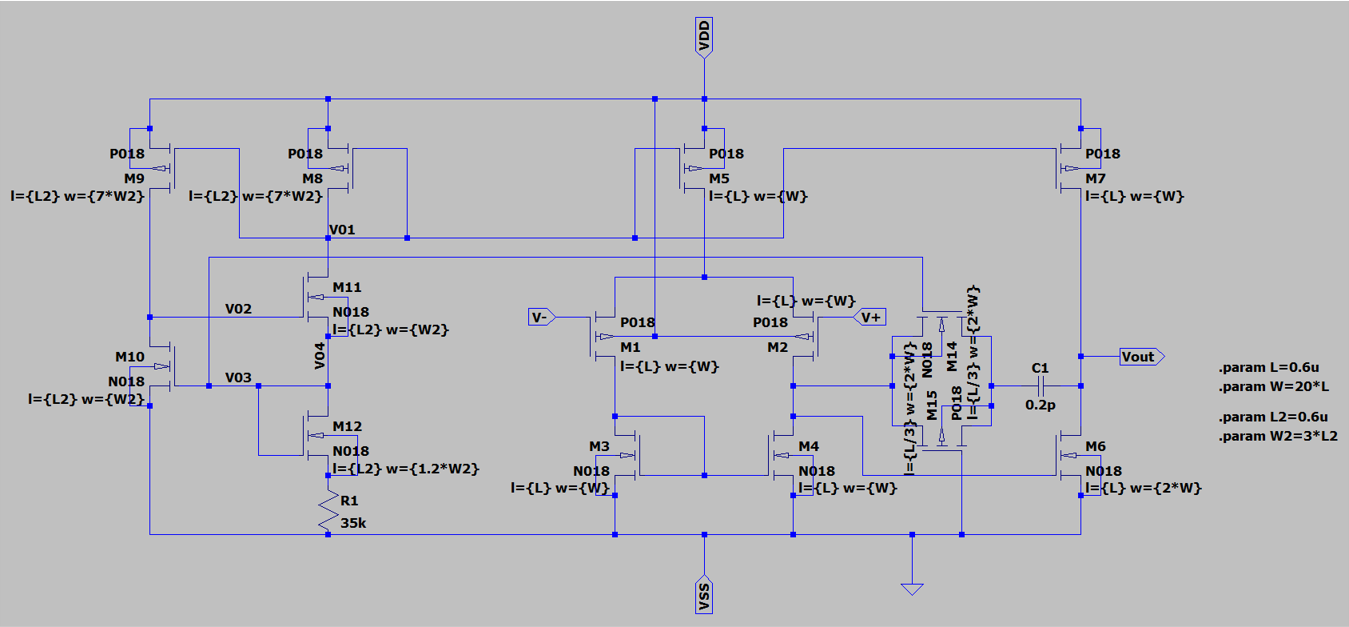
\includegraphics[width = \linewidth]{opamp-improve-2}
    \caption{การเปลี่ยนวงจรสร้างกระแสอ้างอิงเพื่อให้มีขนาดของตัวต้านทานที่ลดลง}
    \label{opamp-improve-2}
\end{figure}

ในวงจรเดิม (จากรูปที่~\ref{my_op_amp}) การไบแอสกระแสที่มีค่าต่ำมาก (ประมาณ 0.5 \si{\micro A}) จำเป็นต้องใช้ตัวต้านทานที่ค่าใหญ่ การแก้ปัญหาเบื้องต้นคือการแทนที่ตัวต้านทานนั้นด้วย diode-connected MOSFET ไม่ว่าอย่างไรก็ตาม การทำเช่นนั้นจะทำให้กระแสอ้างอิงถูกรบกวนอย่างมากด้วย PVT variation หรือความเบี่ยงเบนจากค่าปกติที่อาจเกิดขึ้นกับกระบวนการผลิต, แรงดันจากแหล่งจ่าย และอุณหภูมิของวงจร เนื่องจากความต้านทานของ diode-connected MOSFET ขึ้นอยู่กับการเปลี่ยนแปลงดังกล่าวอย่างมาก

\begin{figure}[h]
    \centering
    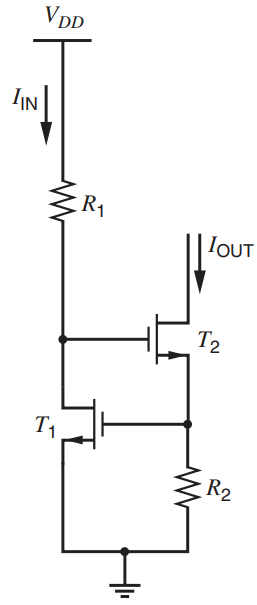
\includegraphics[width = 5cm]{threshold-ref}
    \caption{วงจรสร้างกระแสอ้างอิงแบบ threshold voltage reference}
    \label{threshold-ref}
\end{figure}

การแก้ปัญหาต่อมา คือการเปลี่ยนรูปแบบของวงจรอ้างอิงกระแสให้เป็นแบบ threshold voltage reference แทน ซึ่งได้แสดงในรูปที่~\ref{threshold-ref} \cite{Grey09} เพื่อให้กระแสอ้างอิงเป็นอิสระจากแรงดันจากแหล่งจ่ายและอุณหภูมิของวงจร จากรูปดังกล่าว เมื่อเปรียบเทียบกับรูปที่~\ref{opamp-improve-2} นั่นคือ ทรานซิสเตอร์ T1 และ T2 คือทรานซิสเตอร์ M10 และ M11 ตามลำดับ 

และตัวต้านทาน R2 ในรูปที่~\ref{threshold-ref} ก็คือแทนที่เป็นตัวต้านทาน R1 ต่ออนุกรมกับ diode-connected MOSFET ที่ใช้ M12 ในรูปที่~\ref{opamp-improve-2} 

นอกจากนั้น ตัวสร้างกระแสขาเข้า $I_{IN}$ ในรูปที่~\ref{threshold-ref} สามารถสร้างแทนได้ด้วย current mirror ซึ่งใช้ทรานซิสเตอร์ M8 และ M9 ในรูปที่~\ref{opamp-improve-2} เพื่อให้กระแสของทั้งสองรางถูกผูกไว้อีกทีหนึ่ง

สมการความสัมพันธ์ระหว่าง $I_{IN}$ และ $I_{OUT}$ ของรูปที่~\ref{threshold-ref} สามารถเขียนได้ดังนี้ \cite{Grey09} 
$$I_{OUT} = \frac{V_t + \sqrt{\frac{2I_{IN}}{k'(W/L)_1}}}{R_2}$$

ไม่ว่าอย่างไรก็ตาม การออกแบบวงจรในรูปที่~\ref{opamp-improve-2} ก็ยังมีประสิทธิภาพที่แย่ว่า~\ref{my_op_amp} ซึ่งไม่คุ้มค่ากับการแลกมาของพื้นทีของวงจรที่ใช้บน IC ที่น้อยลง

\chapter{สรุป}

\section{ปัญหา อุปสรรค และข้อเสนอแนะ}

เนื่องจากการทำ Analog Design จำเป็นต้องใช้ความรู้ทางด้านอิเล็กทรอนิกส์อีกมาก ดังนั้นจึงจะต้องอ่านหนังสือเพิ่อค้นคว้าด้วยตัวเอง ซึ่งหนังสือที่แนะนำ เช่น ของ Sedra และ Smith \cite{Sedra15} และจะมีเนื้อหาที่ค่อนข้างลึกบางส่วนที่ในหนังสือ Sedra และ Smith ไม่ได้พูดถึงอีกมาก เช่น สัญญาณรบกวน (Noise) และการออกแบบวงจรสร้างกระแสอ้างอิงที่มีคุณสมบติเพิ่มเติม ฯลฯ ซึ่งแนะนำให้อ่านต่อไปในหนังสือของ Gray \cite{Grey09} และหนังสือการออกแบบวงจร CMOS ของ Razavi \cite{Razavi17}

\backmatter

\chapter*{ภาคผนวก}

ผลการทดลองทั้งหมด: \href{https://mega.nz/folder/Sywj2IDA#qnUAwmZCUlo6esYIEv0eHQ}{คลิกที่นี่}

วงจรและโค้ดทั้งหมดที่ใช้ในการจำลองวงจร: \href{https://github.com/nutchanonj/LTSpice_with_Python}{คลิกที่นี่}

\section*{Code สำหรับการวัดค่าที่เกี่ยวกับผลตอบสนองเชิงความถี่ของอัตราขยายแบบวงเปิด ได้แก่ DC Gain, Crossover Frequency และ Phase Margin}

\begin{singlespace}
\lstinputlisting[language=Python]{codes/1_AC_Sweep.py}
\end{singlespace}

\section*{Code สำหรับการวัดการใช้พลังงานของวงจร}

\begin{singlespace}
\lstinputlisting[language=Python]{codes/2_Power.py}
\end{singlespace}

\section*{Code สำหรับการทดสอบสัญญาณรบกวนของวงจร}

\begin{singlespace}
\lstinputlisting[language=Python]{codes/3_Noise.py}
\end{singlespace}

\section*{Code สำหรับการทดสอบ Settling Time}

\begin{singlespace}
\lstinputlisting[language=Python]{codes/4_Settling_Time.py}
\end{singlespace}

\section*{Code สำหรับการทดสอบ Total Harmonic Distortion}

\begin{singlespace}
\lstinputlisting[language=Python]{codes/5_Fourier.py}
\end{singlespace}

\bibliographystyle{plain}
\bibliography{reference}

\end{document}

